\documentclass[xcolor=dvipsnames]{beamer}

\useoutertheme{infolines} 
\usetheme[height=7mm]{Berkeley}
\usecolortheme[named=Cerulean]{structure} 
\setbeamertemplate{items}[circle]
\setbeamertemplate{navigation symbols}{} 

\usepackage{hyperref}
\usepackage{graphicx} % Needed to resize tables
\usepackage{colortbl} % Used to color table cells
\usepackage{textcomp}
\usepackage[utf8]{inputenc} % For Jérôme ;-)

\usepackage{listings}
\lstset{basicstyle=\textbf\ttfamily,
  commentstyle=\textnormal\textbf\ttfamily,
  showstringspaces=false,
  language=bash,
  basicstyle=\footnotesize,
  frame=leftline,
  fillcolor=\color{cyan},
  keywordstyle=\color{blue},
  resetmargins=true,
  framexleftmargin=-3mm,
  framexrightmargin=3mm,
  backgroundcolor=\color{gray!20}
}

% TODO add shorthand and update sidebar to remove them 
\title[]{Next-Gen Cloud Computing and DevOps with Docker Containers}
\author[]{Hamilton Turner\\{\small \url{hamiltont@gmail.com}}}
\date[March 2014]{March 12, 2014}

% Conditional pause. Either does nothing or forces a pause
\newcommand{\cpause}{}
%\newcommand{\cpause}{\pause}

\begin{document}

\begin{frame}
\maketitle
\end{frame}

\section{Who Am I?}
\begin{frame}
  \frametitle{Who am I?}

  Who am I?
  \begin{itemize}
    \item Ph.D. Candidate at Virginia Tech
      \cpause
      \begin{itemize}
      \item Defending in Fall 2014
      \cpause
      \end{itemize}
    \item Member of Magnum Research Group (http://www.magnum.io/)
      \begin{itemize}
      \item We focus on mobile and cloud applications
      \end{itemize}
  \end{itemize}
  \cpause

  How do I use Docker? 
  \begin{itemize}
    \item Stress test 100+ web apps, without installing natively \cpause
    \item Manage computer cluster for research group \cpause
    \item Personal playground for learning new technologies 
  \end{itemize}
\end{frame}

\section{The DevOps Challenge}
\begin{frame}{DevOps Challenges: The Matrix From Hell}
  \note{Take a look at the current situation of development in many companies}
  \note{Note that developers will primarily be interested in what's happening inside the container. Operations may primarily be interested in what's happening outside the container-start container->runQA}
  
  \resizebox{\linewidth}{!}{% Resize table to fit within \linewidth horizontally
  \begin{tabular}{|l|l|l|l|l|l|l|}
  \hline
  \cellcolor{blue!25}django web frontend            & ?         & ?           & ?         & ?       & ?                       & ?                        \\ \hline
  \cellcolor{blue!25}node.js async API              & ?         & ?           & ?         & ?       & ?                       & ?                        \\ \hline
  \cellcolor{blue!25}background worker tasks        & ?         & ?           & ?         & ?       & ?                       & ?                        \\ \hline
  \cellcolor{blue!25}SQL Database                   & ?         & ?           & ?         & ?       & ?                       & ?                        \\ \hline
  \cellcolor{blue!25}distributed DB, big data tools & ?         & ?           & ?         & ?       & ?                       & ?                        \\ \hline
  \cellcolor{blue!25}message queue                  & ?         & ?           & ?         & ?       & ?                       & ?                        \\ \hline
  ~                              & \cellcolor{red!25}my laptop & \cellcolor{red!25}your laptop & \cellcolor{red!25}QA system & \cellcolor{red!25}staging & \cellcolor{red!25}production on Cloud VM & \cellcolor{red!25}production on bare metal \\ \hline
  \end{tabular}}

  \cpause
  \begin{itemize}
  \item Each environment looks different \cpause
  \item Different developer needs \cpause
  \item Different operations environments \cpause
  \end{itemize}

  The `Big Question'
  \begin{itemize}
  \item How do we make all these environments identical?!
  \end{itemize}

  \vspace{1cm}
  {\footnotesize Credit: Jérôme Petazzoni at \url{http://www.slideshare.net/jpetazzo/introduction-docker-linux-containers-lxc}}
\end{frame}

\section{Beyond VMs}
\begin{frame}{Review of Virtual Machines}
  \note{Like any good academic, I have to provide at least a short background section}
  \note{Other partial solutions exist - chef, ansible, puppet, etc}
  
  Virtual Machines are one current solution

  \begin{columns}
  \column{0.5\textwidth}
  \begin{itemize}
    \item An `entire computer' is executed as a program
    \item No developer's local system has to be modified
    \item The entire VM disk image can be shared  
    \item No more differences between dev and production environments!
    \item This is great! ....Right?
  \end{itemize}

  \column{0.5\textwidth}
  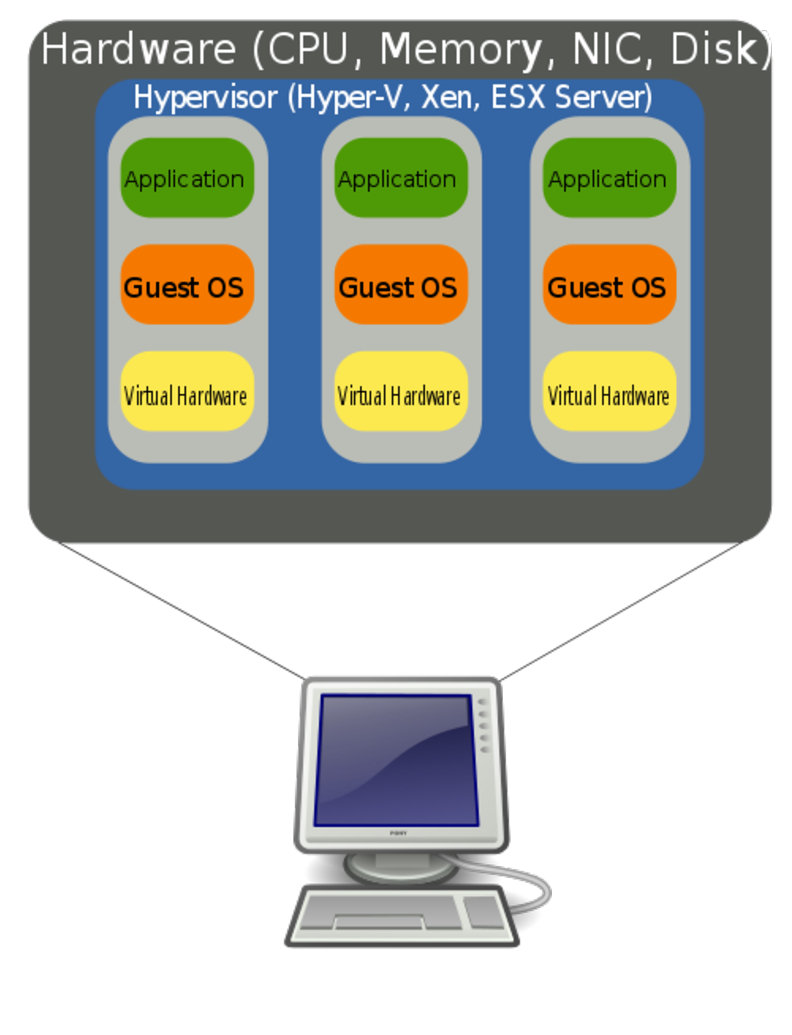
\includegraphics[width=\textwidth]{figures/virtualization.pdf}
  \end{columns}

\end{frame}


\begin{frame}{Comparison of Docker Containers And VMs}
    
  \note{Reproducibility: Union filesystem also natively supports diff}
  \centering
  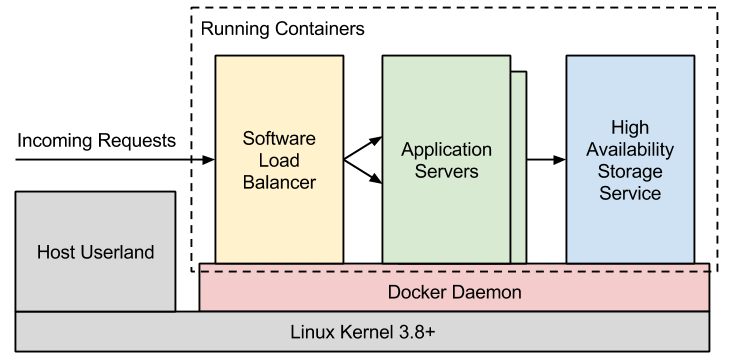
\includegraphics[width=0.6\textwidth]{figures/overview.png}

  {\tiny Credit: quay.io - A Secure Hosting Solution For Private Docker Repositories}\cpause

  \vspace{5mm}

  \resizebox{\linewidth}{!}{% Resize table to fit within \linewidth horizontally
    \begin{tabular}{l|l|l}
    ~                               & Docker Container         & Virtual Machine         \\ \hline
    Avg Host Resources Consumed     & \cellcolor{green!20}Low                      & High                    \cpause \\
    Clean Startup Time              & \cellcolor{green!20}seconds                  & minutes/hours           \cpause \\
    Environment (FS) Sharing        & \cellcolor{green!20}Small (Union filesystem) & Large (Entire Snapshot) \cpause \\
    Environment Reproducibility     & \cellcolor{green!20}High                     & Moderate (AWS image)    \cpause \\
    Software Modifications Needed?  & Perhaps (one process)    & \cellcolor{green!20}Unlikely                \cpause \\
    Attack Surface                  & Untested                 & \cellcolor{green!20}Small                   \cpause \\
    System Monitoring               & \cellcolor{green!20}Use Linux Tools          & Custom systems          \\
    \end{tabular}%
    }




\end{frame}

\section{The How of Docker}
\begin{frame}{The How of Docker}

Docker shares the kernel with the host, uses Linux namespaces+cgroups+union filesystems to isolate
  \begin{columns}
  \column{0.5\textwidth}
    \begin{itemize}
    \item process trees (PIDs) \cpause
    \item mounts (mnt) \cpause
    \item network  (net) \cpause
    \item inter-process communication (ipc) \cpause
    \item user accounts (user) \cpause
    \end{itemize}
  \column{0.5\textwidth}
    \begin{itemize}
    \item hostnames (utc) \cpause
    \item memory \cpause
    \item CPU \cpause
    \item Disk access (blkio) \cpause
    \item Device access (devices) \cpause
    \end{itemize}
  \end{columns}
  \cpause

  \vspace{8mm}
  Summary: Docker combines and standardizes a number of existing Linux components (kernel 3.8$+$)

\end{frame}
  

\begin{frame}{The How of Docker, Union Filesystem Version}

\begin{columns}
\column{0.4\textwidth}
  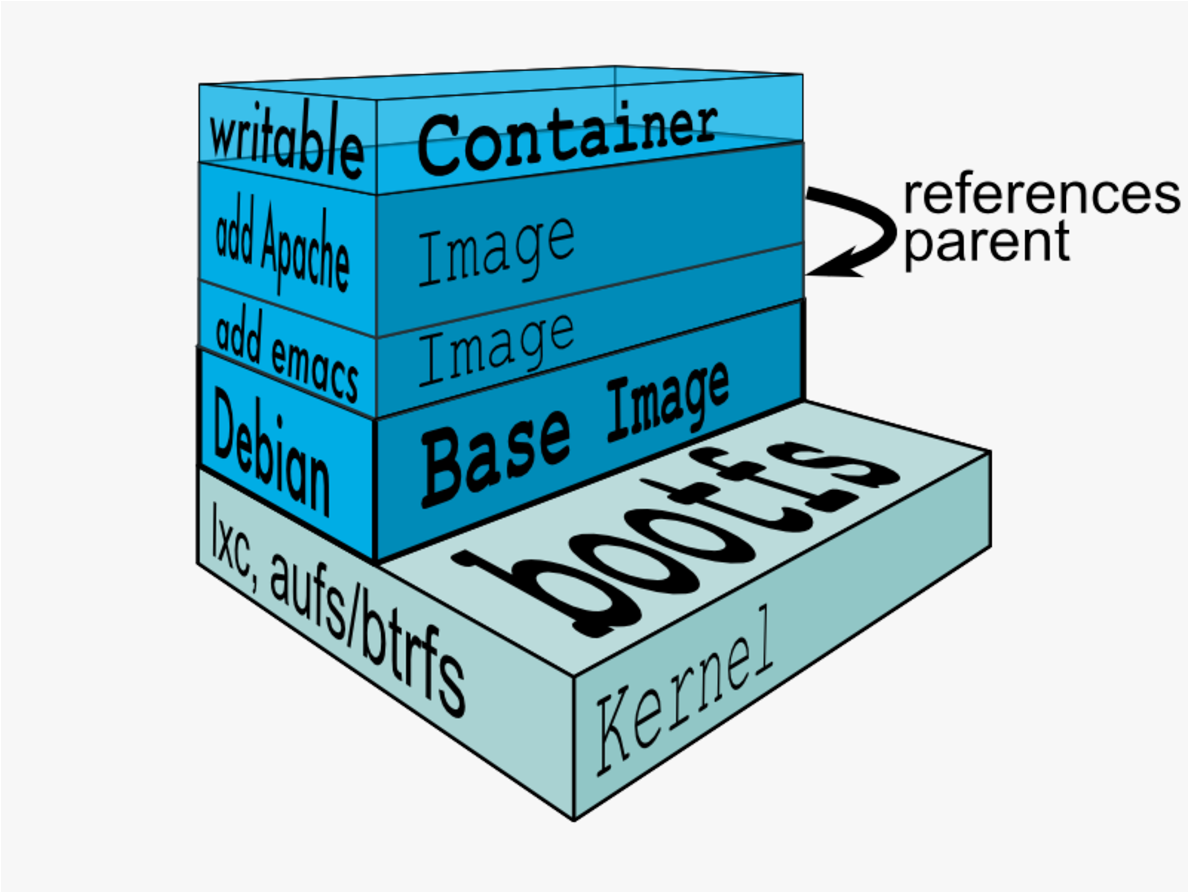
\includegraphics[width=\textwidth]{figures/union-fs.pdf}
\column{0.6\textwidth}
  \begin{itemize}
  \item Each \textit{layer} of the FS is mounted on \textbf{top} of prior layers \cpause
  \item The first layer is the \textit{base image} \cpause
  \item Current base images include debian, ubuntu, busybox, fedora, cent os, etc \cpause
  \item Each read-only layer is called an \textit{image} (A layer is just a collection of files and folders!) \cpause
  \item The top layer is the only modifiable layer - it's termed the \textit{container} \cpause
  \end{itemize}
\end{columns} 

\end{frame}


\section{Docker 101}
\begin{frame}[fragile]
  \frametitle{Docker 101: Run Interactive Container}

  \begin{lstlisting}
  $ sudo docker run -i -t ubuntu /bin/bash
  \end{lstlisting}
  \cpause

  \begin{itemize}
  \item sudo : Docker has to be run as root! \cpause
  \item run : we are running a container \cpause
  \item -i -t : we want a \textbf{terminal} (stdin and stdout), and we want to be connected to those so we can \textbf{interact} with the continer \cpause
  \item ubuntu : The base image for this container \cpause
  \item /bin/bash : Let's run bash \cpause
  \end{itemize}


  \begin{lstlisting}
  $ sudo docker run -i -t ubuntu /bin/bash
  root@03711559d57d:/# cat /etc/*release*
  DISTRIB_ID=Ubuntu
  DISTRIB_RELEASE=12.04
  DISTRIB_CODENAME=precise
  DISTRIB_DESCRIPTION="Ubuntu 12.04 LTS"
  root@03711559d57d:/# exit
  \end{lstlisting}

\end{frame}


\begin{frame}[fragile]
  \frametitle{Docker 101: Run Non-Interactive Container}

  Flags \textbf{-i} and \textbf{-t} are good for interacting with a container, but for
  scripting or long-running tasks, you'll want to use detached (\textbf{-d}) mode

  \cpause
  \begin{lstlisting}
  $ sudo docker run -d ubuntu /bin/bash -c "echo hi" 
  94490365f464bab1f009ec0971e1691213b4562dbaeb04b2e33adcbb1190dafa
  $
  \end{lstlisting}

  \cpause
  Odd things:
  \begin{itemize}
  \item There was no `hi' \cpause
  \item You were given this long string \cpause
  \item You are back at your original shell, even though you ran bash \cpause
  \end{itemize}

  In detached mode, docker immediately returns a container ID. This ID can 
  be used to fetch container stdout, check container status, stop the container, etc

\end{frame}

\begin{frame}[fragile]
  \frametitle{Docker 101: Run Non-Interactive Container, Part Two}

  Ok, let's see what's happening using our container ID

  \begin{lstlisting}
  $ sudo docker run -d ubuntu /bin/bash -c "echo hi"
  d2026870efedf09e29dbea146d399e60493e9dd0ebbf6124347d60d801e295fd
  $ sudo docker logs d2026870efedf09e29dbea146d399e60493e9dd0ebbf6124347d60d801e295fd
  hi
  \end{lstlisting}
  \cpause

  Container ID's can be referenced by unique prefix too

  \begin{lstlisting}
  $ sudo docker logs d202
  hi
  \end{lstlisting}
  \cpause

  \textbf{docker ps} shows you what containers are running \cpause

  \begin{lstlisting}[basicstyle=\tiny]
   $ sudo docker ps
   CONTAINER ID IMAGE         COMMAND               CREATED        STATUS    
   d2026870ef   ubuntu:12.04  /bin/bash -c while t  1 minute ago   Up 1 min  
  \end{lstlisting}    
\end{frame}


\begin{frame}[fragile]
  \frametitle{More on Container IDs}

  \vspace{-2mm}
  Typically, you will want to store the ID \cpause

  \begin{lstlisting}[basicstyle=\tiny]
   $ MY_ECHO=$(sudo docker run -d ubuntu /bin/bash 
     -c "echo hi")
   $ sudo docker logs $MY_ECHO
   hi
  \end{lstlisting}

  \vspace{-2mm}
  \begin{itemize}
  \item Detached Mode (e.g. \textbf{docker run -d}) \cpause
    \begin{itemize}
    \item Docker run response is the container ID \cpause
    \item To capure the output, we use \ttfamily{\$(...)} \cpause
    \item This output is stored into variable \ttfamily{MY\_ECHO}, and later retrieved with \ttfamily{\$MY\_ECHO} \cpause
    \end{itemize}
  \vspace{-1mm}
  \item Interactive Mode (e.g. \textbf{docker run -i -t})
    \begin{itemize}
    \item Run container, modify, then exit. Container is now stopped \cpause
    \item Use \textbf{docker ps -a} to show \textit{all} containers, incl. stopped ones \cpause
    \item Or use \textbf{docker ps -l -q} to show the \textit{last} container ID 
    \cpause
    \end{itemize}
  \end{itemize}

  \vspace{-2mm}
  \begin{lstlisting}[basicstyle=\tiny]
   $ sudo docker ps -a
   CONTAINER ID IMAGE         COMMAND               CREATED        STATUS    
   d2026870ef   ubuntu:12.04  /bin/bash -c while t  1 minute ago   Exit 0  
   $ sudo docker ps -q -l
   d2026870ef
  \end{lstlisting} 
  \cpause

  \vspace{-1mm}
  Note: Docker now supports container \textbf{names}

\end{frame}

\begin{frame}[fragile]
  \frametitle{Storing A Container For Reuse \\(a.k.a. Building an Image)}

  \begin{columns}
  \column{0.7\textwidth}
    \begin{itemize}\itemsep0em
      \item Recall: the \textbf{container} filesystem is the final union with a stack of images

      \item \textbf{docker commit} converts this container filesystem into an \textbf{image}

      \item The \textbf{image} can then be used to run other containers
    \end{itemize}
  \column{0.3\textwidth}
    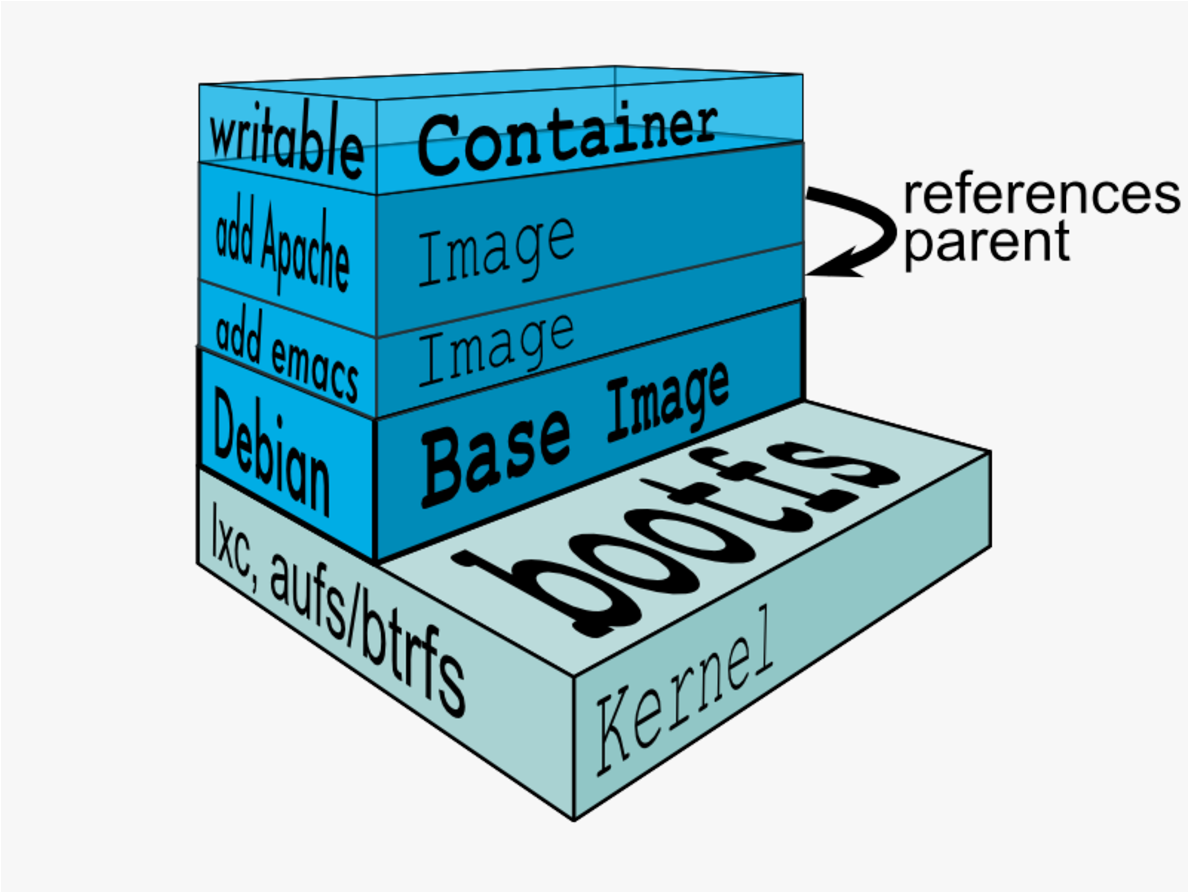
\includegraphics[width=\textwidth]{figures/union-fs.pdf}
  \end{columns} 
  \cpause

  \begin{lstlisting}
  $ APP=$(sudo docker run -d ubuntu /bin/bash -c 
    ``echo hi > config.out'')
  $ sudo docker commit $APP hamiltont/myapp
  $ sudo docker run -i -t hamiltont/myapp /bin/bash
  root@3a1f0c28b822:/# cat config.out
  hi
  \end{lstlisting}
  \cpause

  If you could share this image...then others could build new containers based on this image!

\end{frame}


\begin{frame}[fragile]
  \frametitle{Sharing An Image For Reuse}

  \begin{itemize}
    \item Images can be shared using a registry \cpause

    \item \textbf{docker push} and \textbf{docker pull} \cpause

    \item There is a public registry available, or your company can host it's 
    own private registry {\tiny Check out quay.io} \cpause

    \item If \textbf{docker run} does not find the image locally, it will 
    automatically search known registries \cpause
    
  \end{itemize}

  \begin{lstlisting}
  $ sudo docker push hamiltont/myapp
  $ sudo docker pull hamiltont/myotherapp
  \end{lstlisting}
  \cpause

  \begin{itemize}
    \item The \textbf{images} subcommand can be used to list local images
  \end{itemize}
  \cpause
  
  \begin{lstlisting}[basicstyle=\tiny]
   $ sudo docker images
   REPOSITORY            TAG     IMAGE ID     CREATED         VIRTUAL SIZE
   hamiltont/myapp       latest  d100b411c51e 2 minutes ago   204.4 MB
   hamiltont/myotherapp  latest  7cb2d9010d39 11 days ago     410.6 MB
   ubuntu                12.04   9cd978db300e 5 weeks ago     204.4 MB
   ubuntu                latest  9cd978db300e 5 weeks ago     204.4 MB
  \end{lstlisting}

\end{frame}

\begin{frame}[fragile]
 \frametitle{Benefits of Using Union Filesystems For Images}

  \begin{itemize}
    \item Hypothetical:
      \begin{itemize}
      \item I run a ubuntu container, make changes, and exit \cpause
      \item I commit my changes to an image and run \textbf{docker push} \cpause
      \item My colleage wants to \textbf{docker pull} my image \cpause
      \item What do they need to download? \cpause
      \end{itemize}
    \item Answer: 
      \begin{itemize}
      \item Just your changes! \cpause
      \item They have probably already downloaded the ubuntu base image
      \end{itemize}
    \item No inherent need for multi-GB images \cpause
    \item Download only files, not arbitrary filesystem junk \cpause
    \item While YMMV, \\ $80\%$ of images are $\leq50MB$, $95\%$ are $\leq500MB$ 
  \end{itemize}

\end{frame}

\begin{frame}[fragile]
 \frametitle{Linking Host/Container Filesystems}

 \vspace{-2mm}
 A nice seperation of concerns would place application inside the container, logs outside the container. \cpause

 The \textbf{-v} flag can mount a host volume to the container\cpause

 \note{Or...configuration outside the container, application inside}
  \vspace{-1mm}
  \begin{lstlisting}
  $ sudo mkdir /app_logs
  $ sudo docker run -i -t -v /app_logs:/logs ubuntu 
    /bin/bash
  root@842fa9699353:/# cd /logs/
  root@842fa9699353:/logs# echo "My application log" 
    > log.out
  root@842fa9699353:/logs# exit
  $ cat /app_logs/log.out
  My application log
  \end{lstlisting}
  \vspace{-1mm}
  \cpause

  \textbf{-v} can also be used to access configuration on the host
  \cpause

  \vspace{-1mm}
  \begin{lstlisting}
  $ sudo mkdir /app_conf
  $ sudo docker run -i -t -v /app_conf:/etc/app ubuntu 
    /bin/bash
  root@842fa9699353:/# my_app --conf /etc/app
  \end{lstlisting}  

\end{frame}


\begin{frame}[fragile]
 \frametitle{Exposing Container Network Ports}

  Docker container ports are not published unless requested. \cpause

  The \textbf{-p} flag can be used to publish a port \cpause

  \begin{lstlisting}
  $ SERVER=$(docker run -d -p 8000 ubuntu /bin/bash 
    -c `while true; do sleep 5; done')
  $ sudo docker port $SERVER 8000
  0.0.0.0:49158
  \end{lstlisting}
  \cpause

  Breakdown: 
  \begin{itemize}
  \item Run a bash process inside the container, looping indefinitely \cpause
  \item \textbf{-p 8000} caused Docker to find an unused host port and link it with the container-internal port 8000 \cpause
  \item We used the \textbf{port} subcommand to find this public port \cpause
  \item There is nothing listening on port 8000 in the container, so this is 
  kind of boring
  \end{itemize}

\end{frame}


\begin{frame}[fragile]
 \frametitle{Exposing Container Network Ports, Part Two}

  So let's run an actual webserver! \cpause
  
    Method 1: Build my own webserver image
  
    Method 2: Reuse someone else's pre-built image
  \cpause 

  \begin{lstlisting}
  $ WEB_SERVER=$(sudo docker run -t -d 
    -p 8000 hamiltont/python-simplehttpserver)
  $ sudo docker logs $WEB_SERVER
  Serving HTTP on 0.0.0.0 port 8000 ...
  $ sudo docker port $WEB_SERVER 8000
  0.0.0.0:49186
  \end{lstlisting}

  Note: 
  \begin{itemize}
  \item I chose to reuse hamiltont/python-simplehttpserver \cpause
  \item Navigating to \url{http://localhost:49186} will now connect me to the webserver
  \cpause
  \item The container knew what command to run! More on this next...
  \end{itemize}

\end{frame}

\begin{frame}[fragile]
  \frametitle{Building Images with Dockerfiles}

  
  \begin{itemize}
  \item We know how to run a container, modify it, and commit it as an image \cpause
  \item A \textbf{Dockerfile} lists the steps needed to build an images \cpause
  \item Similar to a Makefile \cpause
  \item \textbf{docker build} is used to run a Dockerfile \cpause
  \item Can define default command for \textbf{docker run}, ports to expose, etc
        \cpause
  \end{itemize}

  \centering
  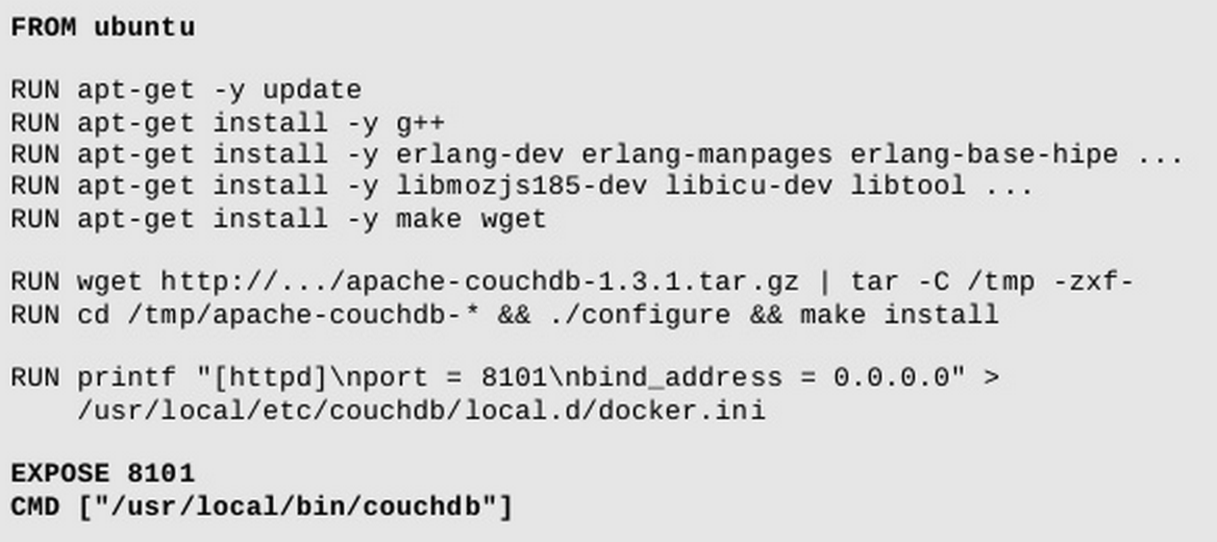
\includegraphics[width=0.8\textwidth]{figures/dockerfile.pdf}
  
\end{frame}


\begin{frame}[fragile]
  \frametitle{Locating Community Images}

  \cpause
  
\includegraphics[width=\textwidth]{figures/docker-index.pdf}

  \begin{itemize}
  \item There are hundreds of community-contributed and/or official images online at \url{http://index.docker.io} \cpause
  \item This is the official registry, you can also host your own
  \item You can also use the \textbf{docker search} subcommand to interact with \url{index.docker.io} \cpause
  \end{itemize}

  \begin{lstlisting}[basicstyle=\tiny]
   $ sudo docker search wordpress
   NAME              DESCRIPTION                                STARS TRUSTED
   ctlc/wordpress                                                 4    [OK]
   jbfink/docker-wor Same as jbfink/wordpress, just a trusted b   2    [OK]
   skxskx/wordpress  Wordpress & SSH in a container.              2
   eugeneware/docker                                              1    [OK]
   tutum/wordpress   Wordpress Docker image - listens in port 80  1    [OK]
   jbfink/wordpress  Wordpress 3.8                                1
  \end{lstlisting}

\end{frame}

\begin{frame}{Docker 101 Review: Topics Covered}  

  \begin{itemize}
  \item Running Docker Containers In Interactive or Detached Mode \cpause
  \item Container IDs (and names) \cpause
  \item Viewing output of detached container (\textbf{docker logs}) \cpause
  \item Committing containers to create images \cpause
  \item Sharing images via push/pull \cpause
  \item Mounting Filesystems From Host inside container \cpause
  \item Exposing container network ports \cpause
  \item Basic concept of Dockerfiles
  \end{itemize}
\end{frame}

\begin{frame}{Docker 101: Things We Didn't Cover}  
  
  \cpause
  \begin{itemize}
  \item Detach from running container, then re-attaching \cpause
  \item Diff'ing filesystems \cpause
  \item Storing container/image as tar file \cpause
  \item Using \textbf{docker kill} to stop a running container \cpause
  \item Deleting unused containers/images \cpause
  \item Examining processes inside container from the host \cpause
  \item Linking containers together (via filesystem or network) \cpause
  \item Trusted builds \cpause
  \item Limiting container memory and CPU consumption \cpause
  \end{itemize}

  \vspace{8mm}
  {\LARGE Any questions at this point? }
\end{frame}

\section{Docker Examples}

\begin{frame}
  \frametitle{A (small) selection of Dockerized Projects}

  \begin{tabular}{p{0.4\textwidth}|p{0.5\textwidth}}
  Data Storage             & Redis, MySQL, MongoDB, memcached                              \\ \hline \cpause
  Server Stacks            & Nginx, Apache+PHP, SSH                                        \\ \hline \cpause
  Development \linebreak Environments & Python, Go, Ruby, Java, Chef/Puppet, node.js, X11+SSH Desktop \\ \hline \cpause
  Blogging / CMS           & Wordpress, Ghost                                              \\ \hline \cpause
  Single-use tool usage    & Redis CLI, Latex, subuser                                     \\ \hline \cpause
  Continuous Integration   & Jenkins, Drone                                                \\ \hline \cpause
  Proxy Software           & Hipache, Nginx/Apache/noje.js                                 \\ \hline \cpause
  PaaS                     & Cocaine (from Yandex), Deis, Flynn, Bowery, Dokku             \\ 
  \end{tabular}
\end{frame}

\begin{frame}[fragile]
  \frametitle{Example: Wordpress}
  \begin{lstlisting}
  # WP=$(docker run -d -p 80 tutum/wordpress)
  # docker port $WP 80
  0.0.0.0:49159
  \end{lstlisting}
  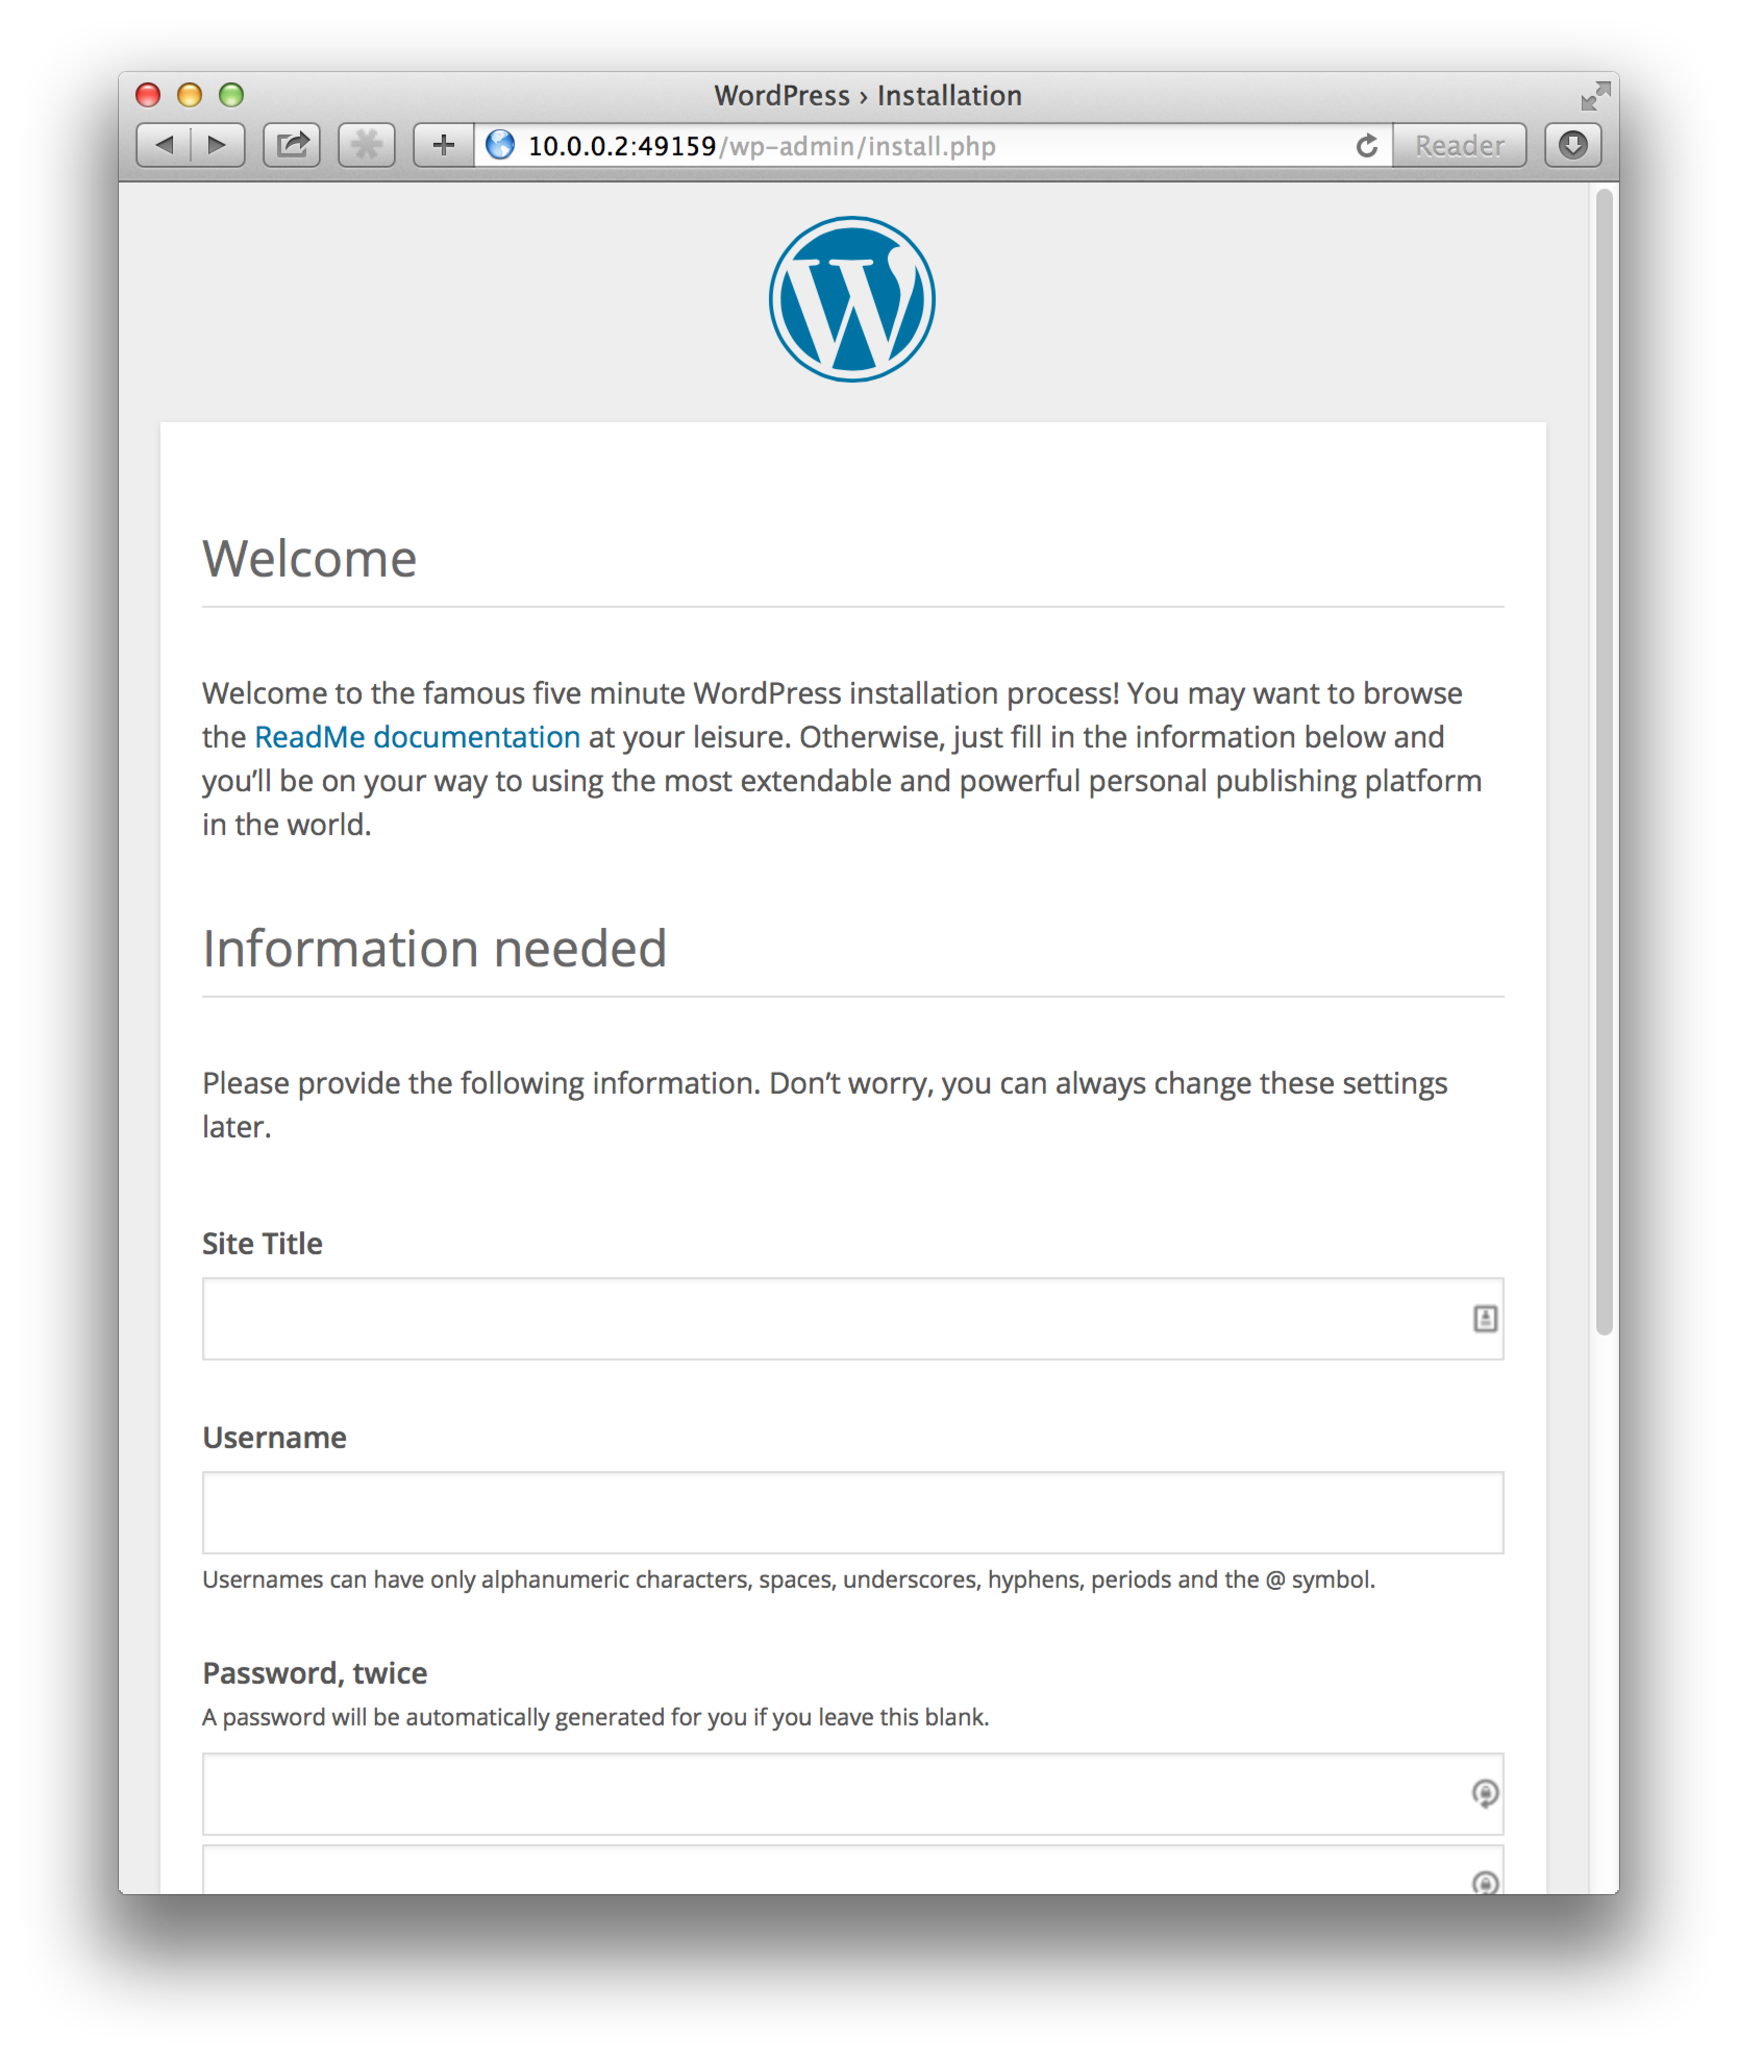
\includegraphics[width=\textwidth]{figures/wordpress.pdf}
\end{frame}

\begin{frame}[fragile]
  \frametitle{Example: Redis Commander Web GUI}
  \begin{lstlisting}[basicstyle=\tiny]
   # RD=$(docker run -d -p 8081 elsdoerfer/redis-commander)
   # docker port $RD 8081
   0.0.0.0:49159
  \end{lstlisting}
  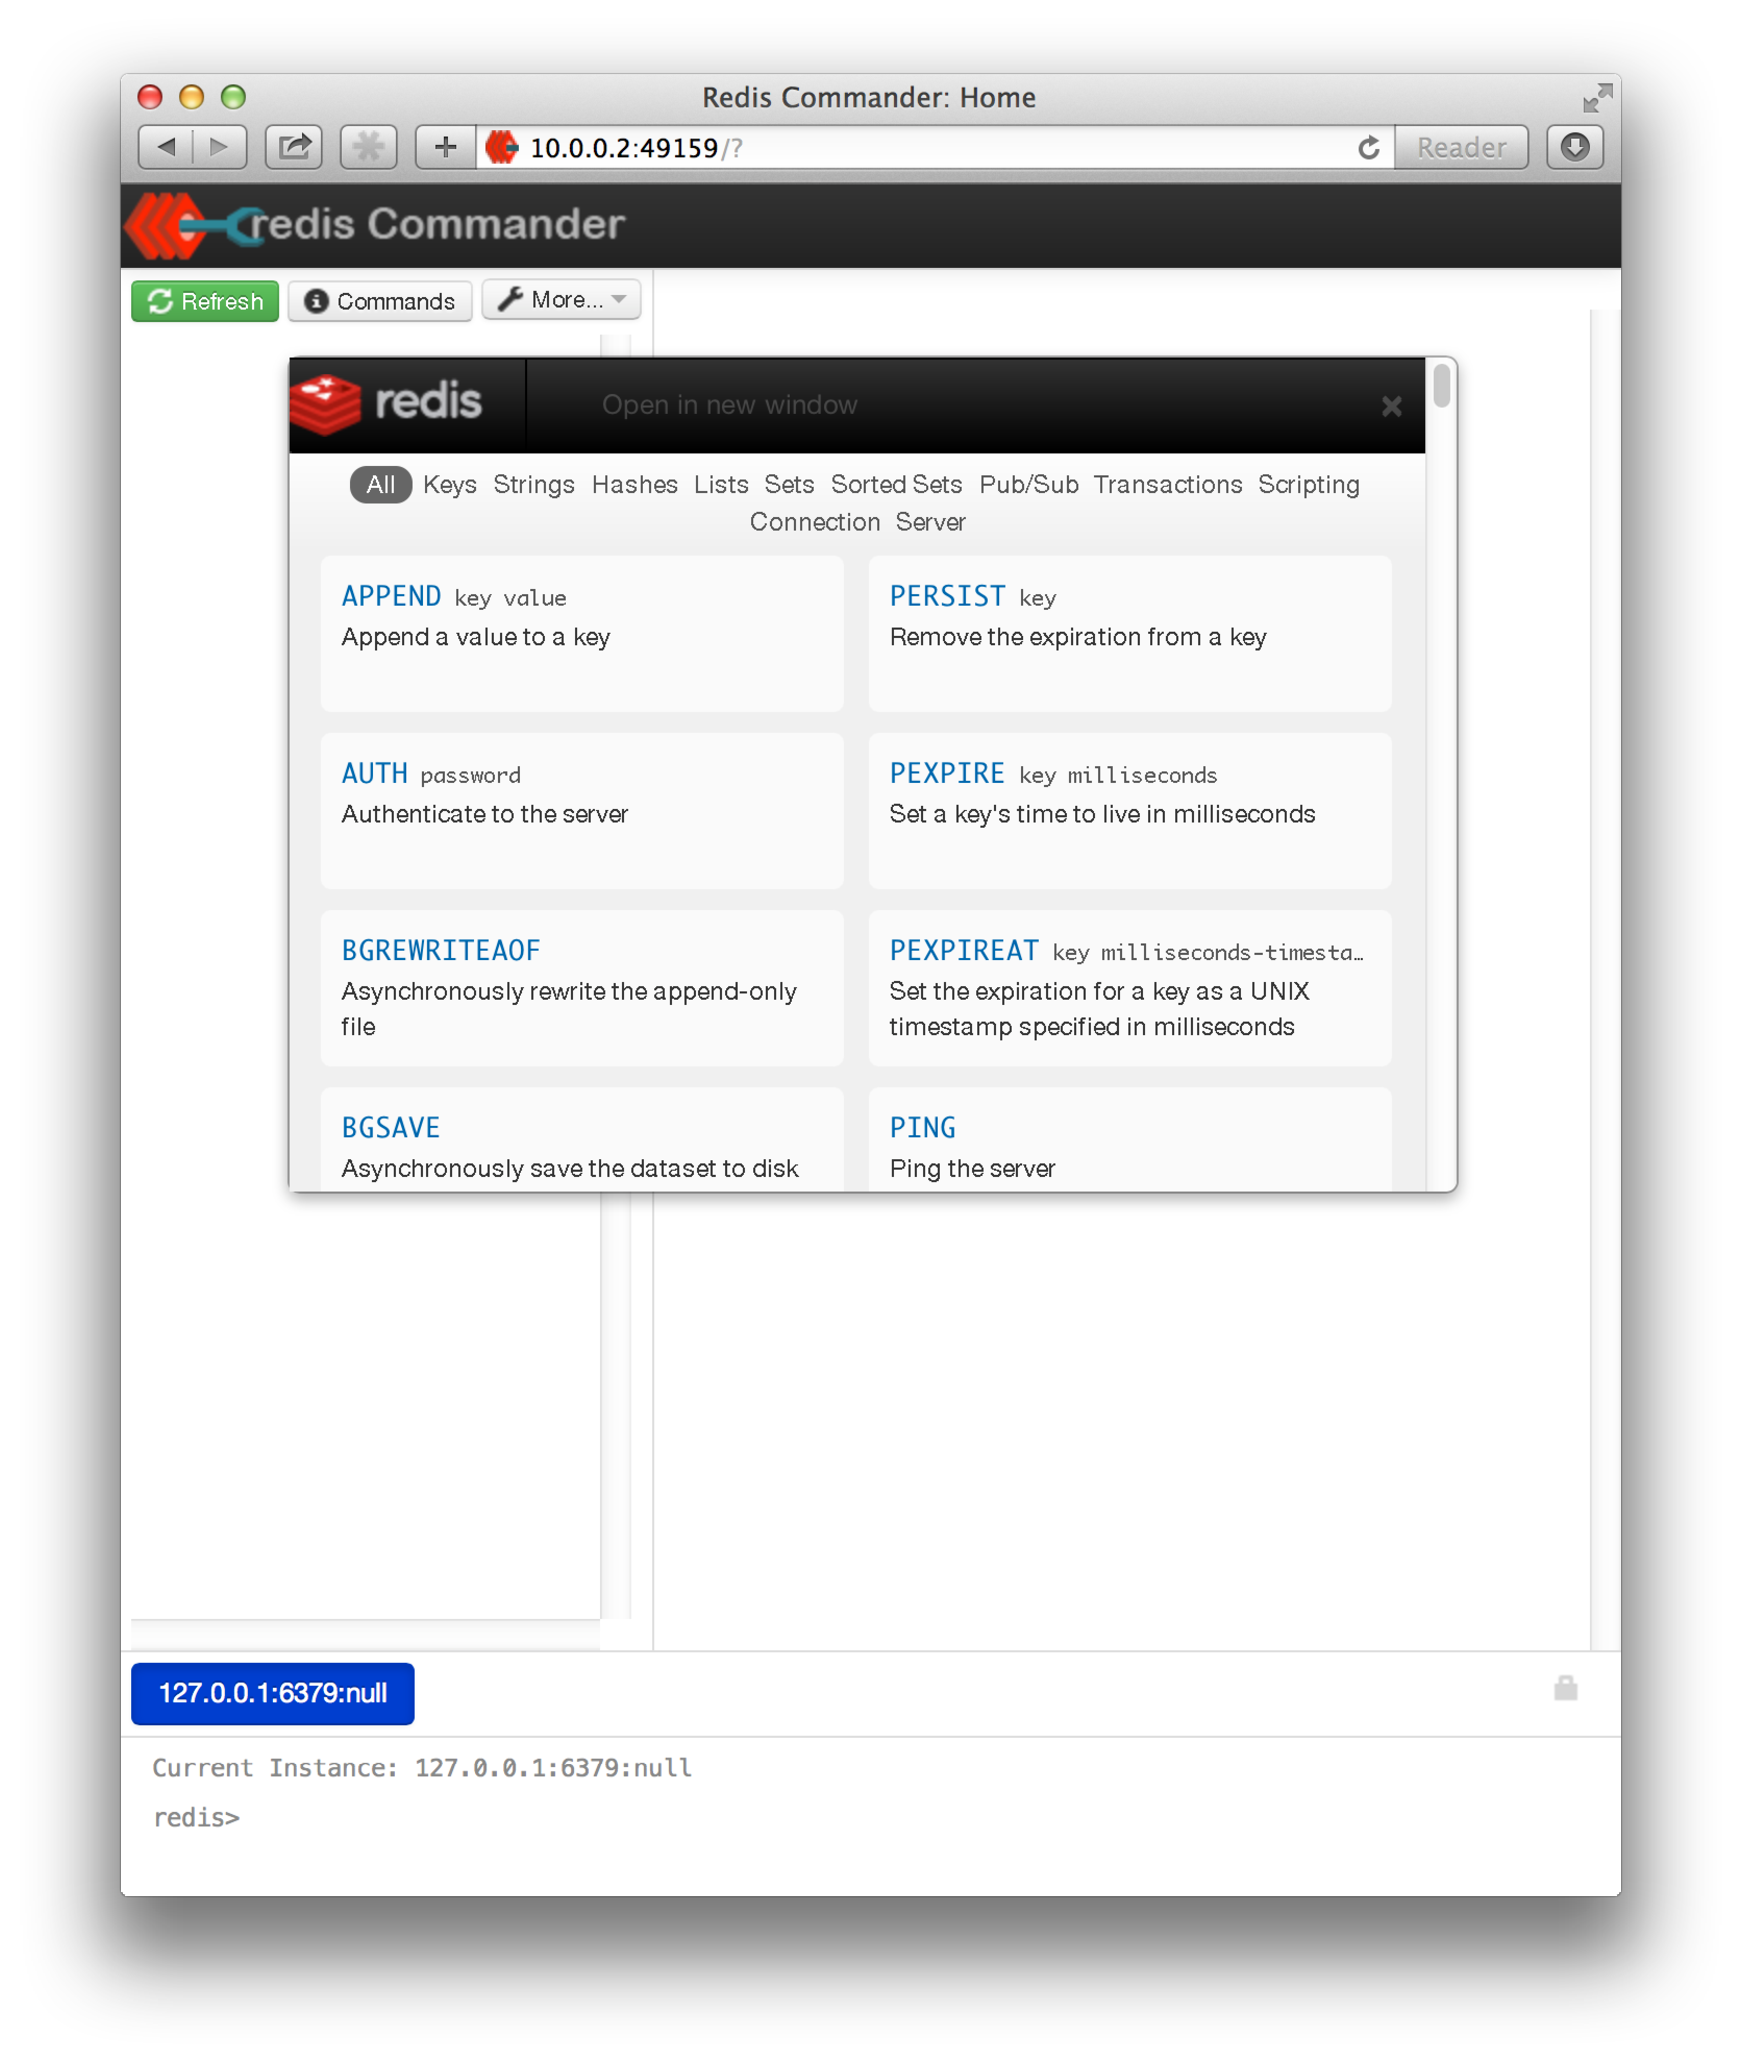
\includegraphics[width=\textwidth]{figures/redis-commander.pdf}
\end{frame}


\begin{frame}[fragile]
  \frametitle{Example: Sandboxed Dev Environment}
  \begin{lstlisting}[basicstyle=\tiny]
   # docker run -t -i -p 22 magglass1/docker-browser-over-ssh
   IP address:     172.17.0.4
   Password: N24DjBM86gPubuEE
   Firefox:  ssh -X webuser@172.17.0.4 firefox
   Google Chrome:  ssh -X webuser@172.17.0.4 google-chrome --no-sandbox
  \end{lstlisting}
  \begin{columns}
  \column{0.5\textwidth}
  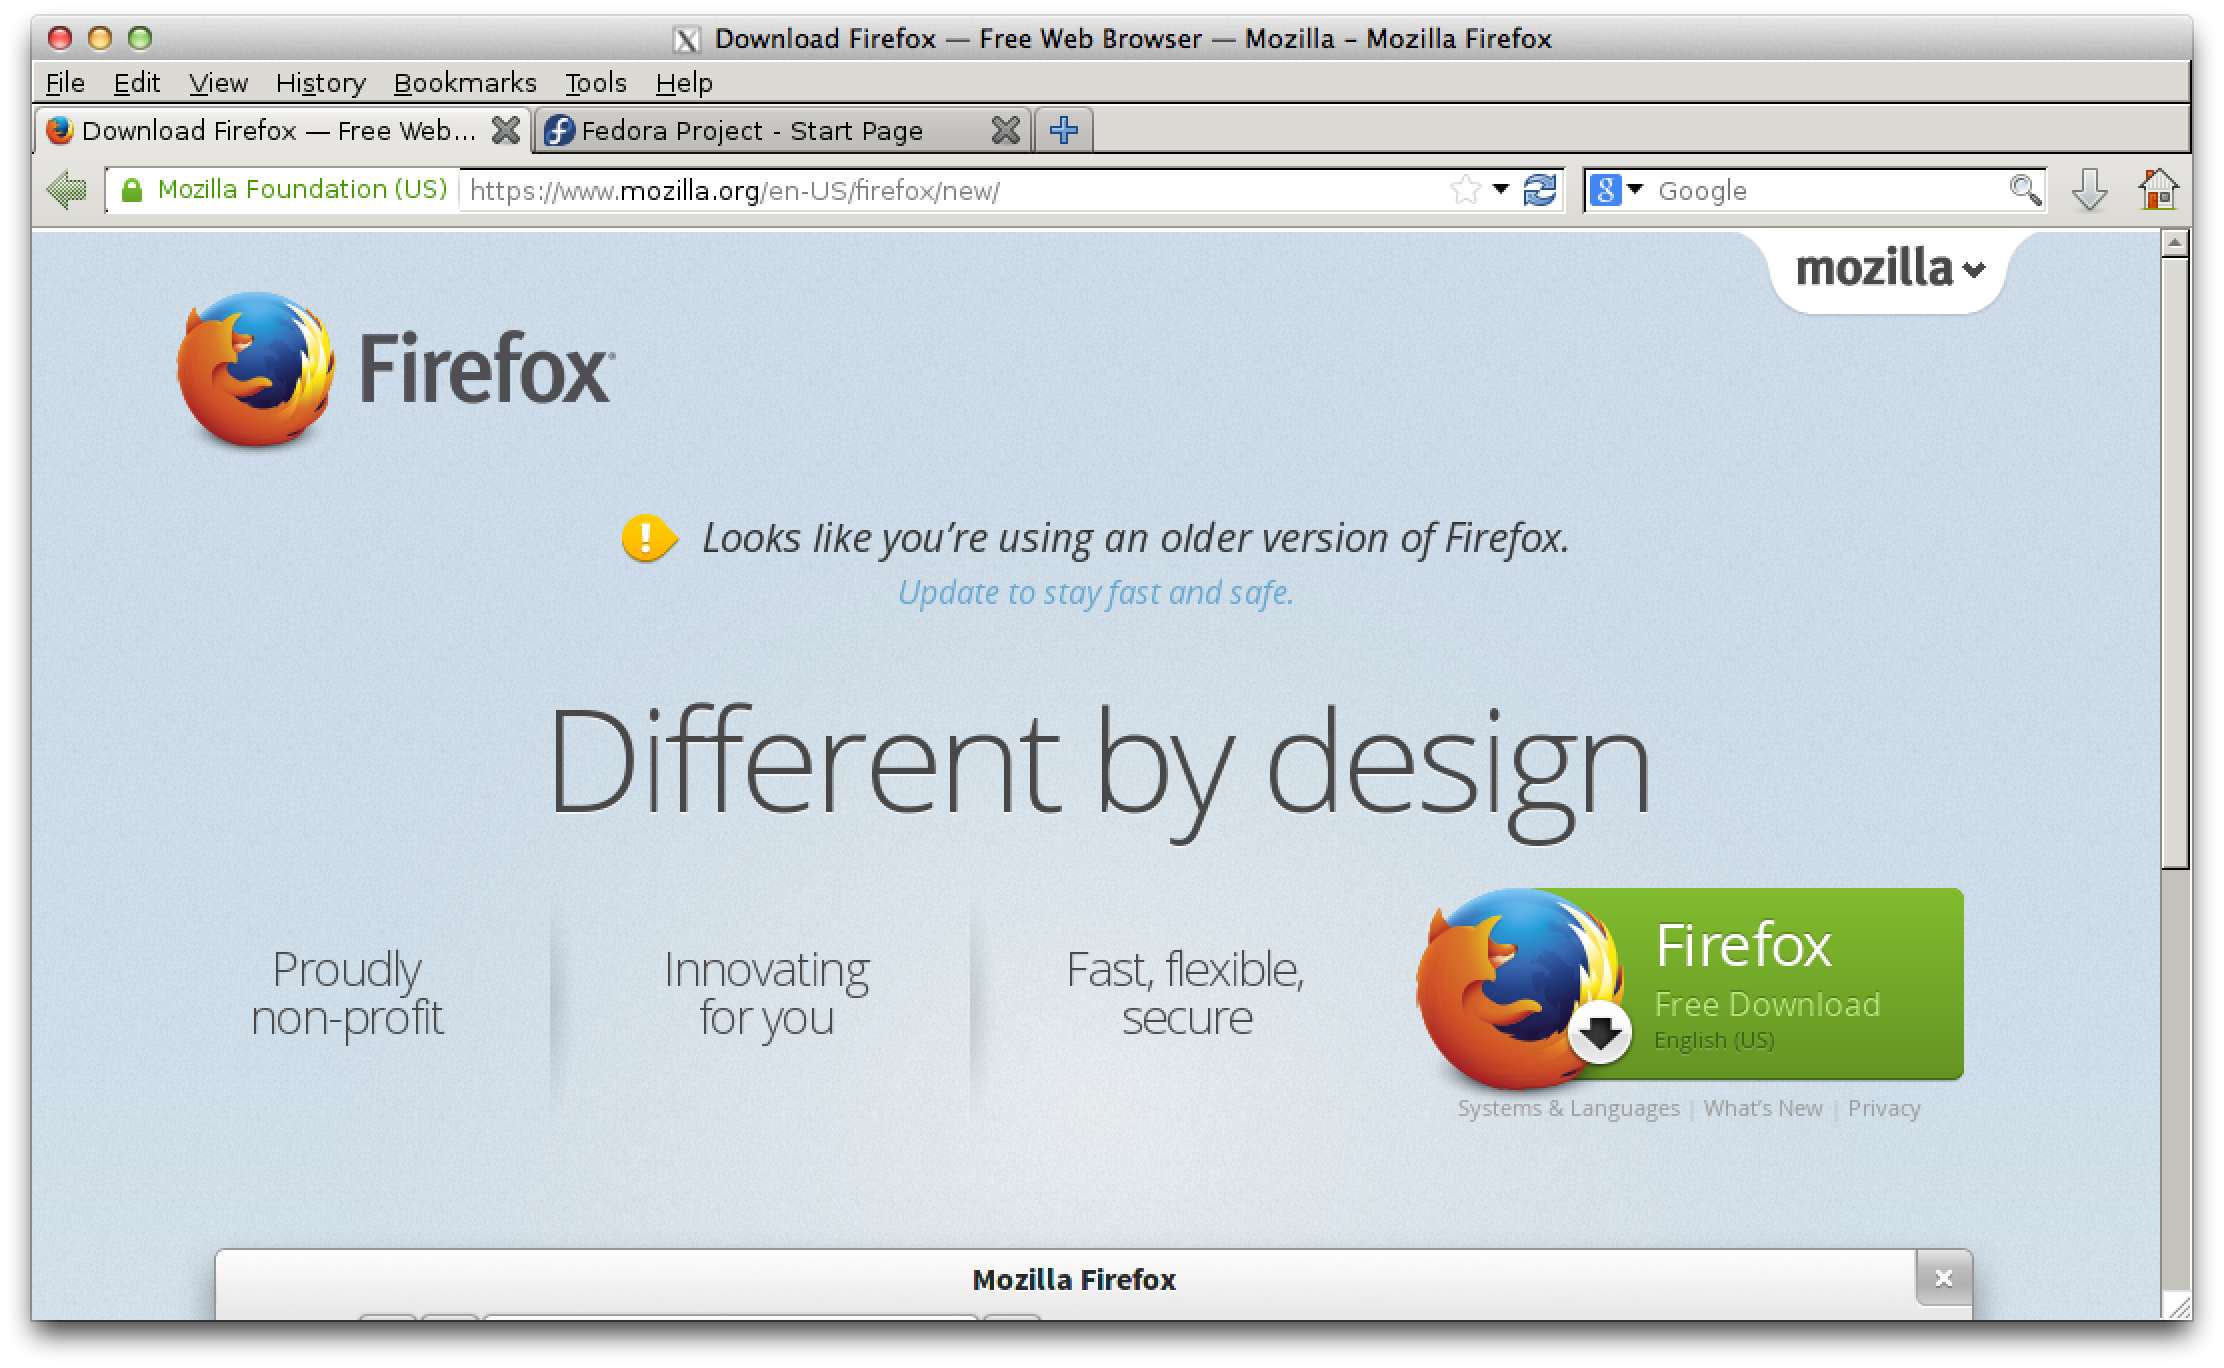
\includegraphics[width=\textwidth]{figures/firefox.png}
  \column{0.5\textwidth}
  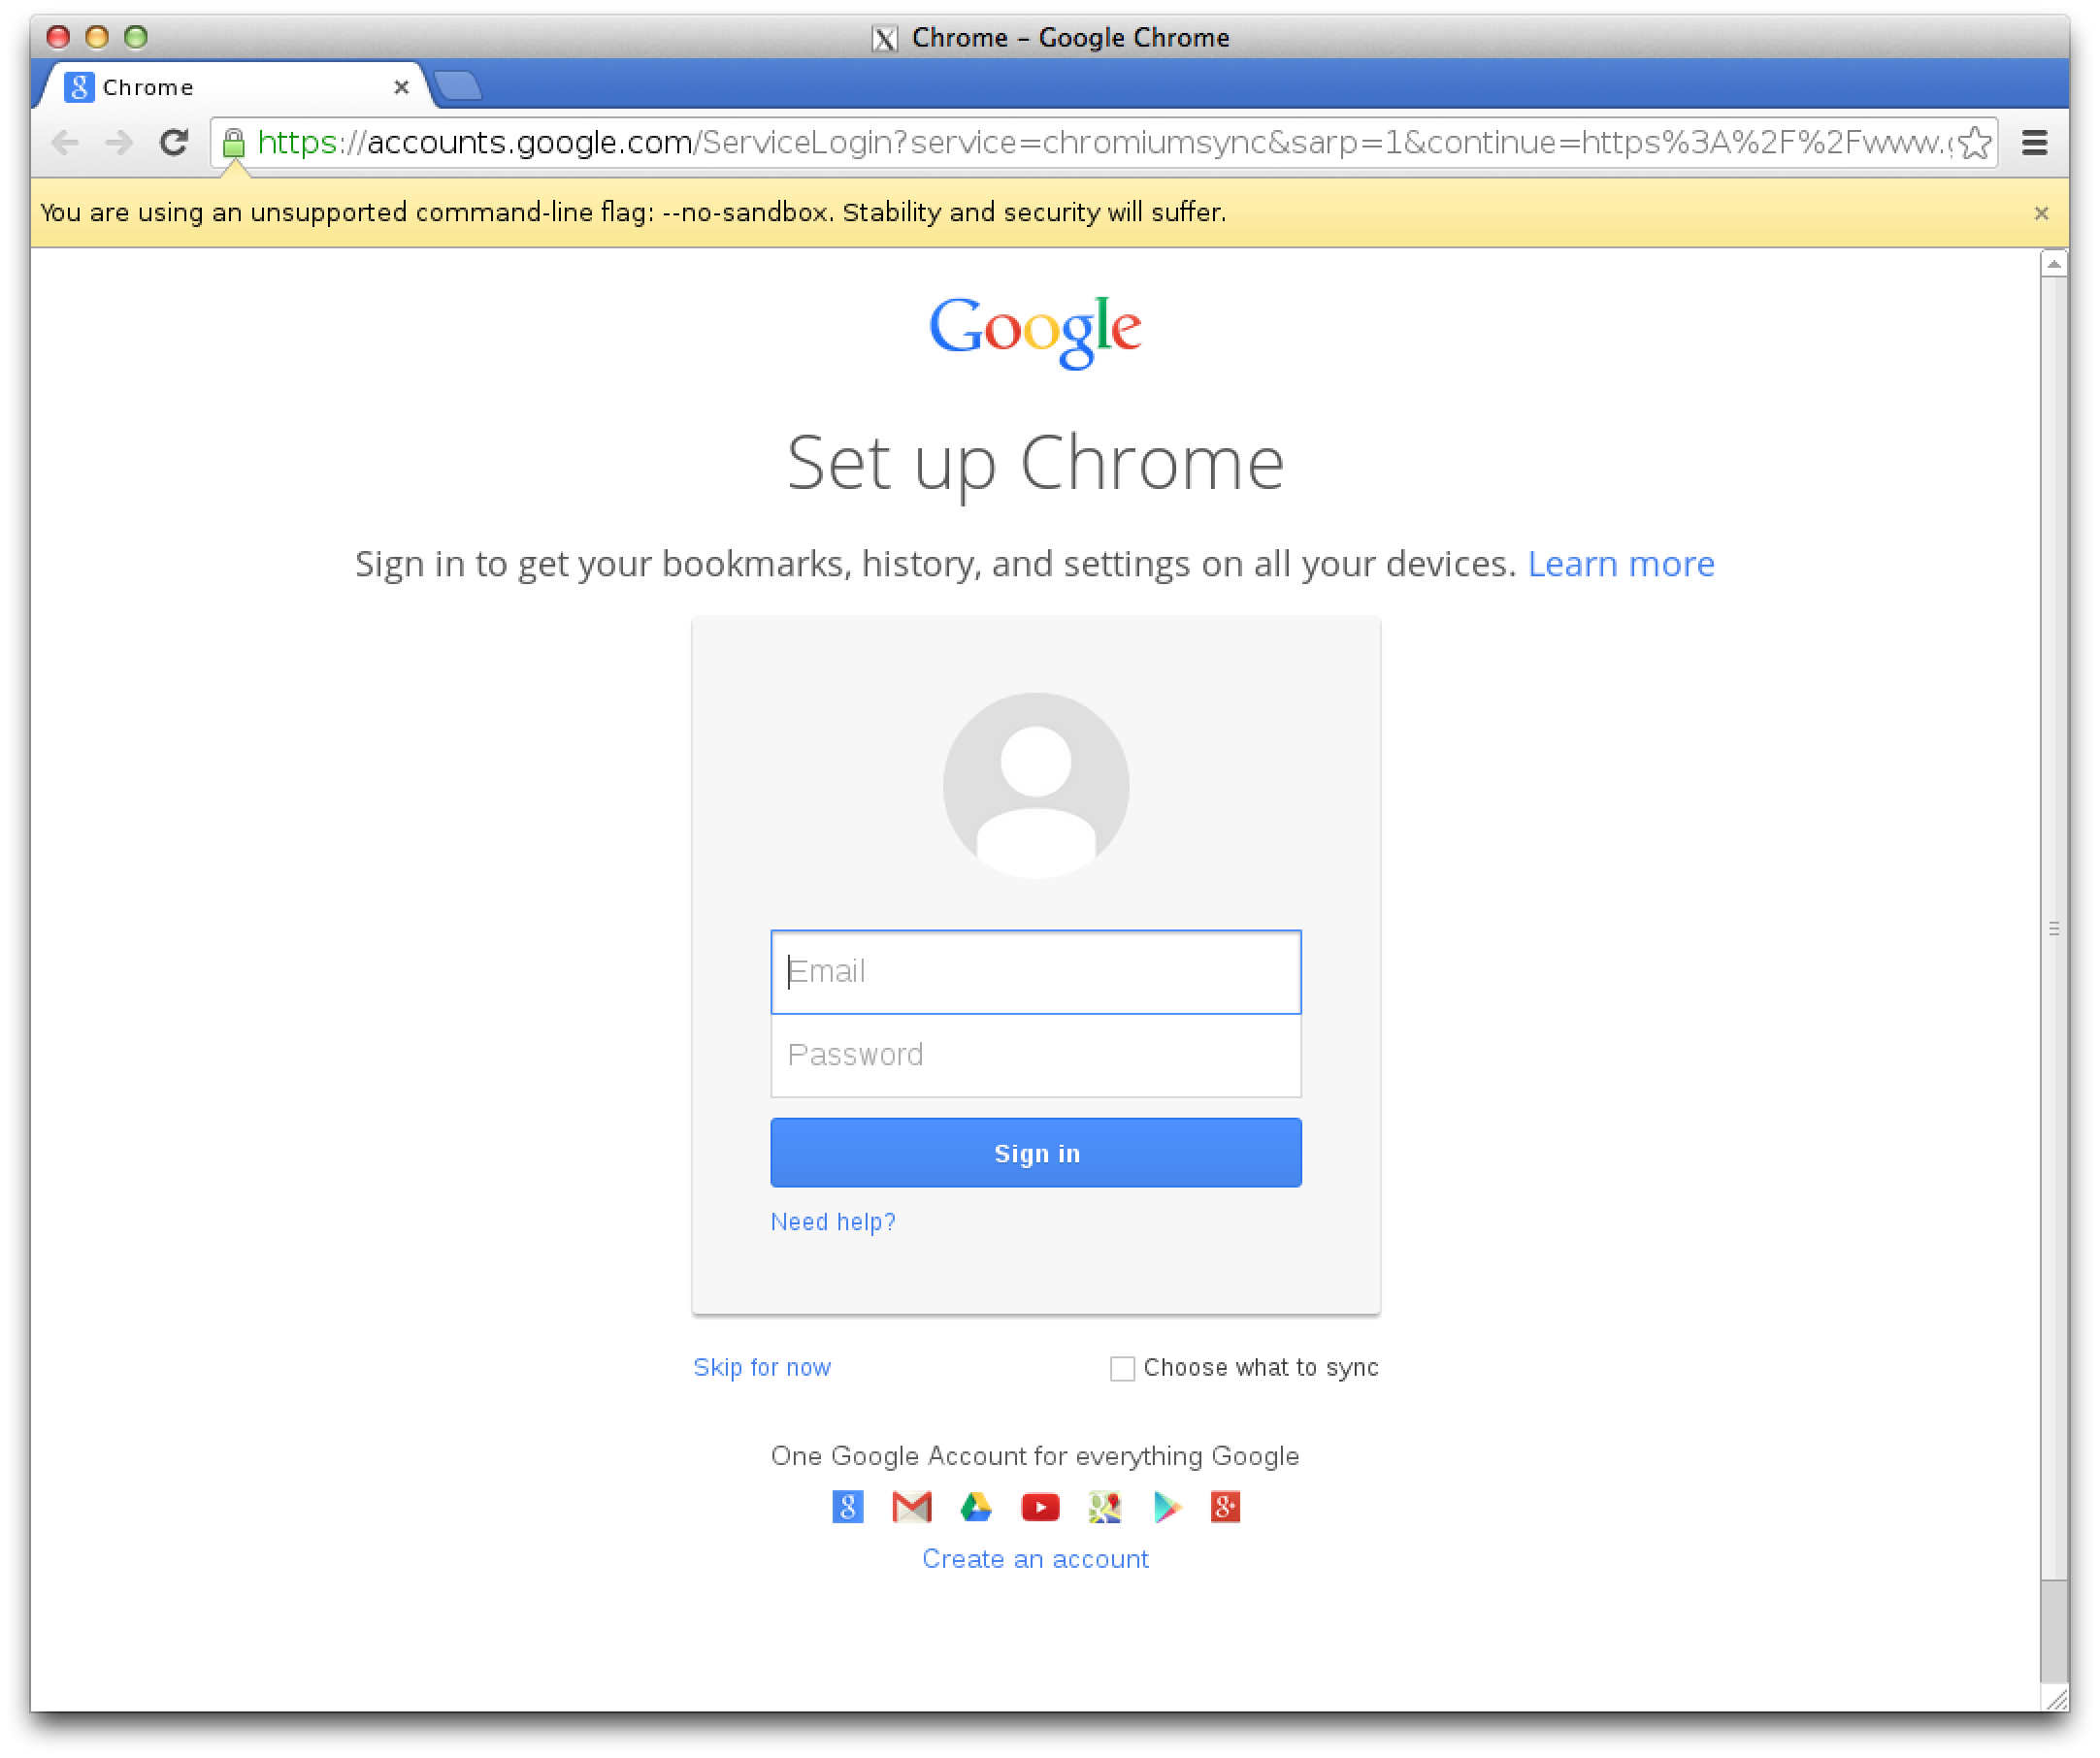
\includegraphics[width=\textwidth]{figures/chrome.png}
  \end{columns}
\end{frame}


\begin{frame}[fragile]
  \frametitle{Example: SSH Server}
  \begin{lstlisting}
  # SSH=$(docker run -d -p 22 dhrp/sshd)
  # docker port $SSH 22
  0.0.0.0:49160
  \end{lstlisting}

  Ok, SSH is running. Now to connect!

\begin{lstlisting}[basicstyle=\tiny]
   $ ssh -p 49161 root@10.0.0.2
   root@10.0.0.2's password:
   Welcome to Ubuntu 12.04 LTS (GNU/Linux 3.11.0-18-generic x86_64)

    * Documentation:  https://help.ubuntu.com/

   The programs included with the Ubuntu system are free software;
   the exact distribution terms for each program are described in the
   individual files in /usr/share/doc/*/copyright.

   Ubuntu comes with ABSOLUTELY NO WARRANTY, to the extent permitted by
   applicable law.

   root@7d45b427eca1:~#
  \end{lstlisting}
  
\end{frame}


\begin{frame}[fragile]
  \frametitle{Example: Continuous Integration}
  \begin{lstlisting}[basicstyle=\tiny]
   # JEN=$($docker run -d -p 8080 --cpu-shares=20 lzhang/jenkins)
   # docker port $JEN 8080
   0.0.0.0:49160
  \end{lstlisting}

  Note: I've limited the CPU shares allowed
  
  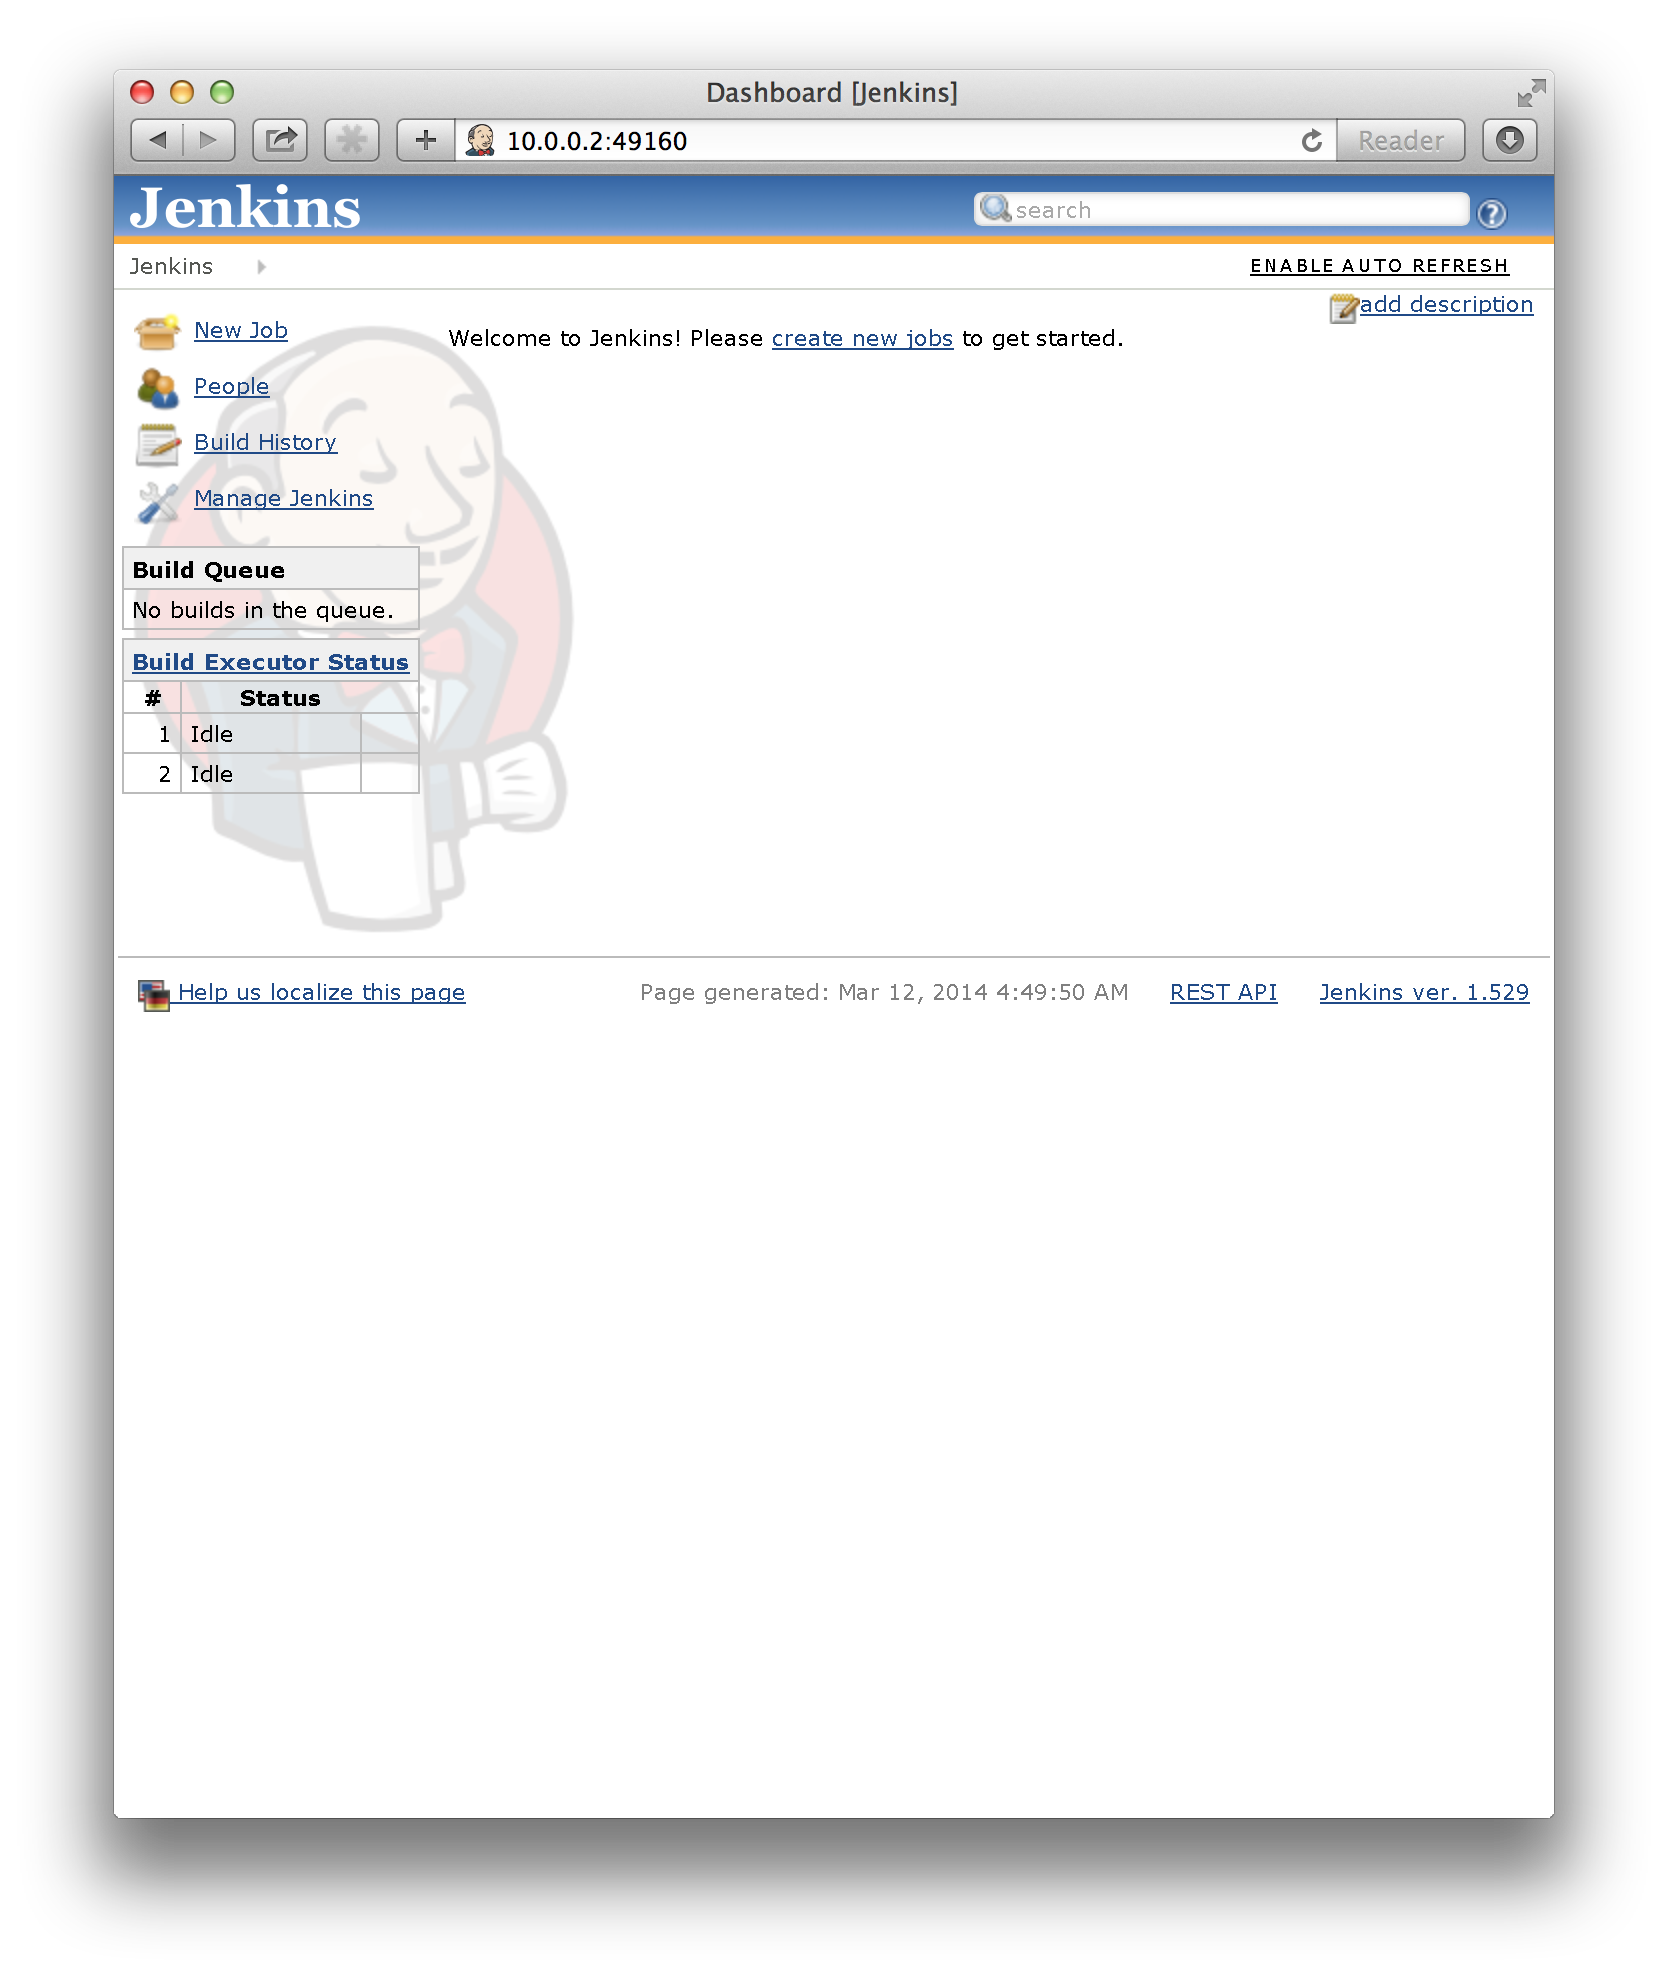
\includegraphics[width=\textwidth]{figures/jenkins.png}
  
\end{frame}


\begin{frame}[fragile]
  \frametitle{Example: Quick Web Server}
  \begin{lstlisting}[basicstyle=\tiny]
   # WEB=$(docker run -d -v /Programming:/www -p 8000 hamiltont/python-simplehttpserver)
   # docker port $WEB 8000
   0.0.0.0:49160
  \end{lstlisting}

  Note: I've mounted my \ttfamily{/Programming} folder to  \ttfamily{/www}
  
  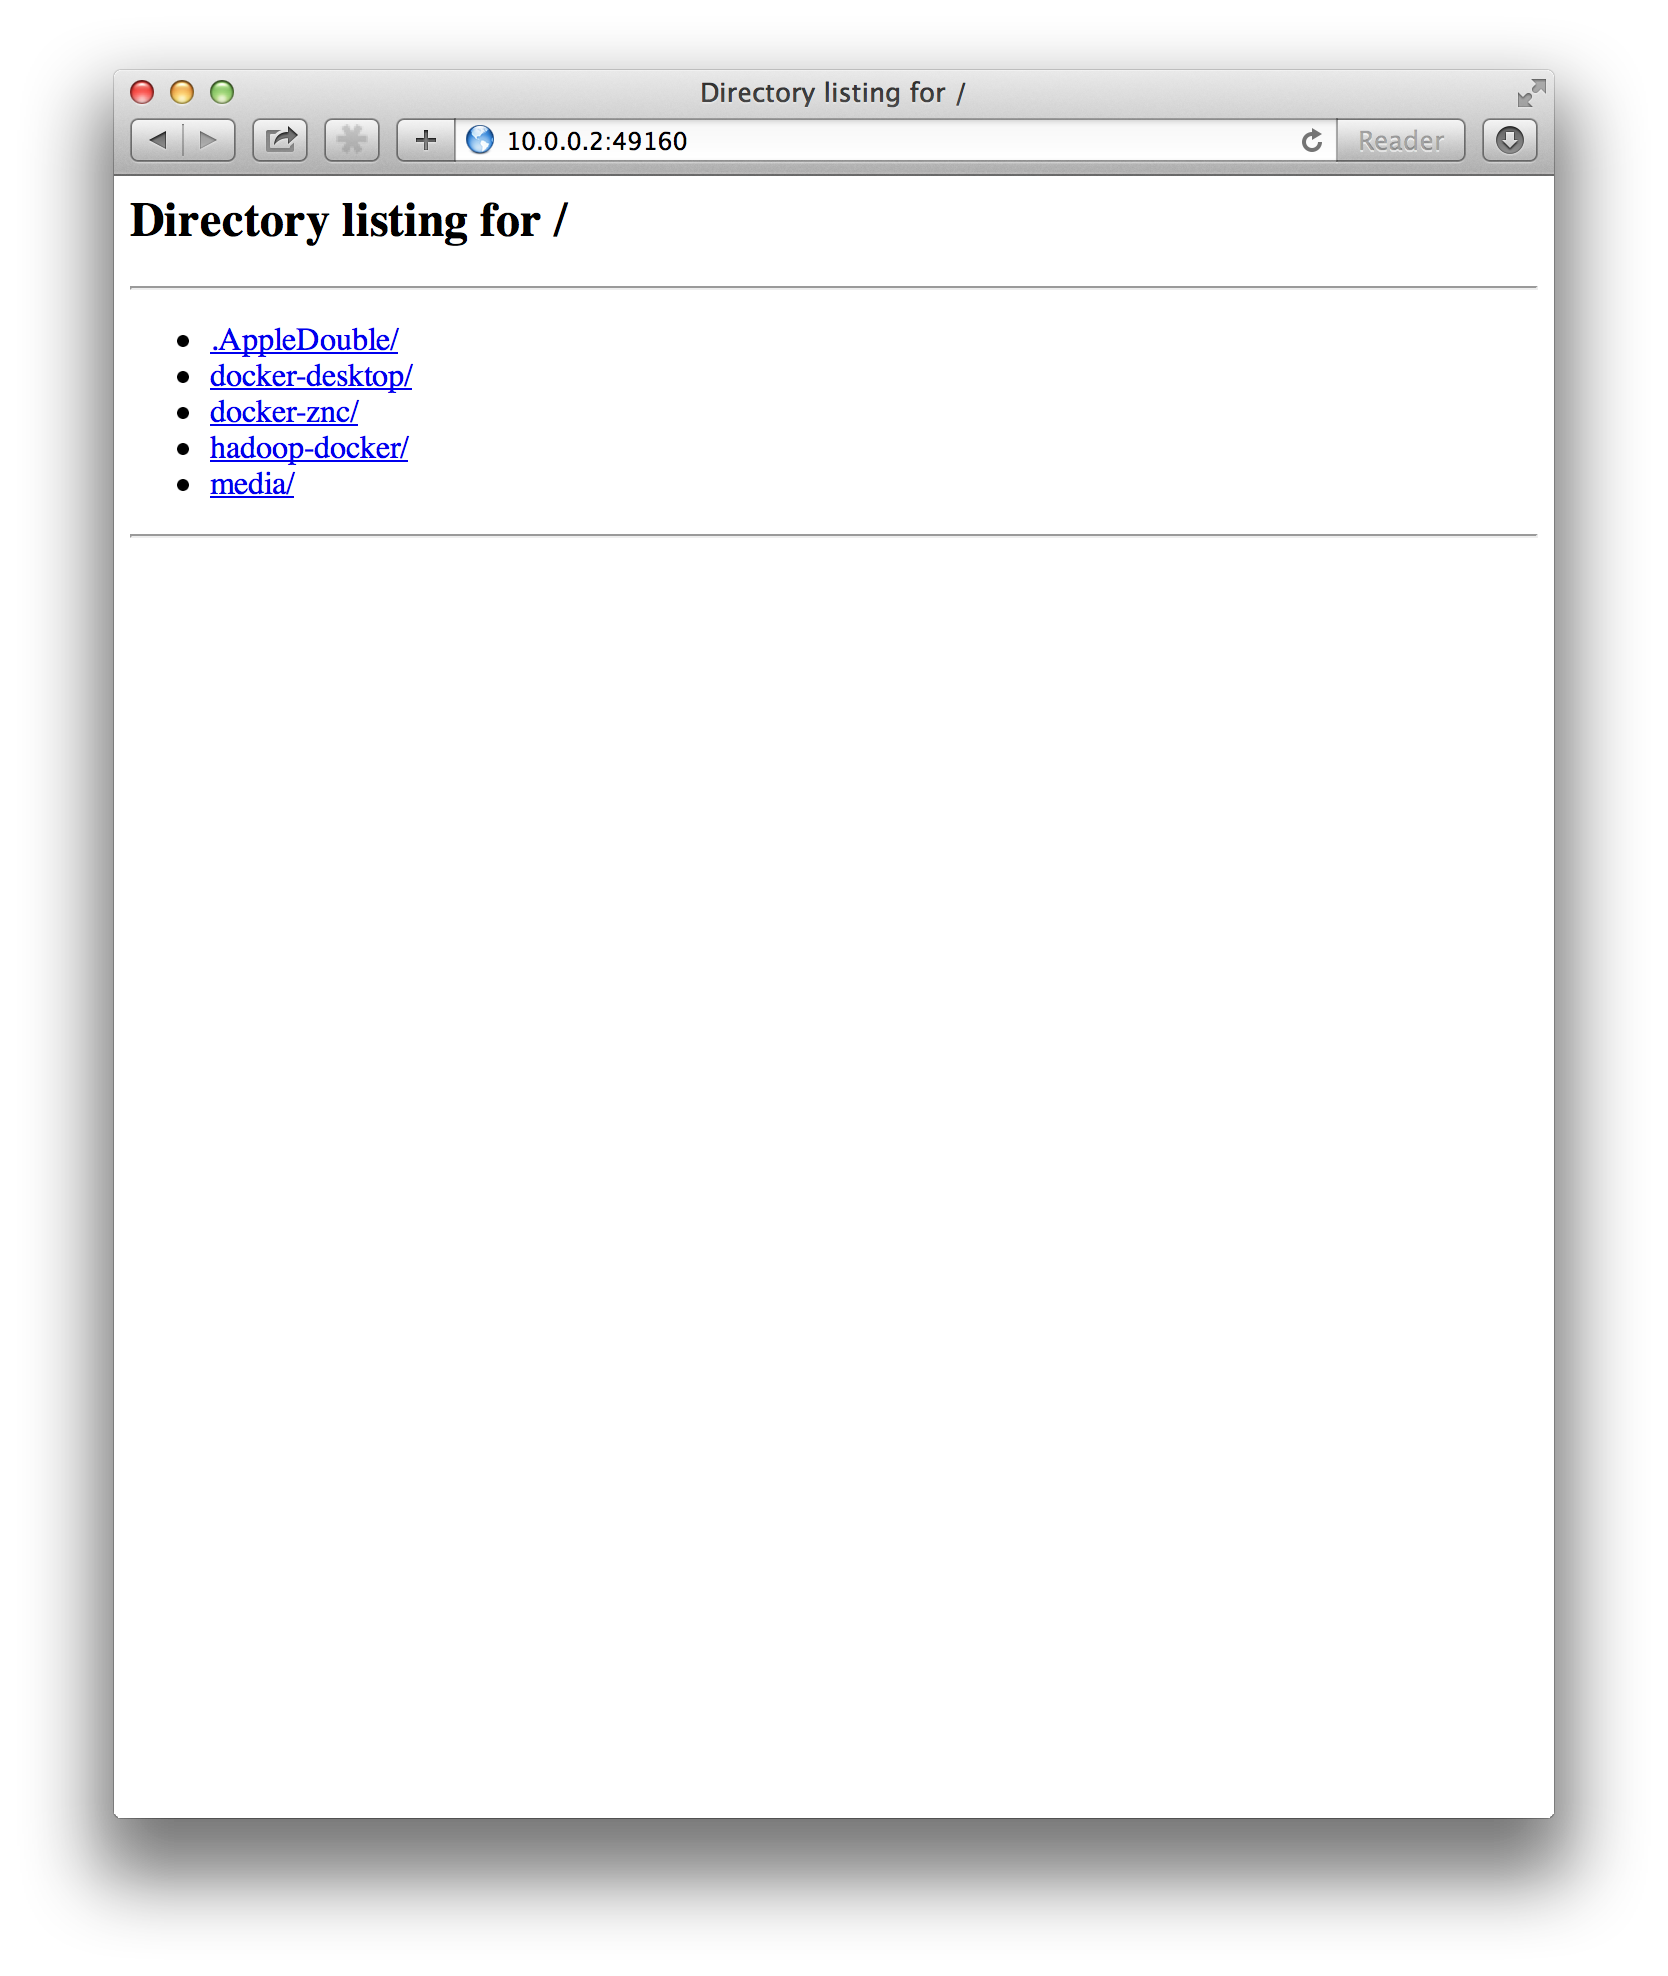
\includegraphics[width=\textwidth]{figures/python-webserver.png}
\end{frame}

\begin{frame}[fragile]
  \frametitle{Example: Using Redis CLI Without Installing It}
  \begin{lstlisting}
  # docker run -i -t crosbymichael/redis-cli -h 
    redis.myhost.com `KEYS *'
  1) "four"
  2) "one"
  3) "two"
  \end{lstlisting}

  \begin{itemize}
    \item Redis is not installed on the host \cpause

    \item I can use complex (and stateful!) commands without modifying the 
    host machine \cpause

    \item I could even pull my dotfiles onto a production machine \cpause

    \item No noticable run delay
  \end{itemize}

\end{frame}


\begin{frame}[fragile]
  \frametitle{Example: Preexisting Automation Tools}
  
  \begin{itemize}
    \item Docker doesn't exclude existing tools like Chef, Puppet, etc \cpause

    \item Current base systems are limited to (mostly) Debian \cpause

    \item Most current automation systems can be used seamlessly \cpause 

    \item But...you no longer have to worry as much about OS updates as the 
    Docker image is static ;-) \cpause
  \end{itemize}

  CentOS+Chef: \cpause
  \begin{lstlisting}
  # docker run -i -t raybeam/chef /bin/bash
  bash-4.1# knife
  ERROR: You need to pass a sub-command 
    (e.g., knife SUB-COMMAND)
  ... <snip>
  \end{lstlisting}

\end{frame}


\section{Docker Limits}

\begin{frame}[fragile]
  \frametitle{Docker Is Not a Panacea: Considerations}

  \begin{itemize}
    \item No Shared Libraries
      \begin{itemize}
      \item The price of process isolation \cpause
      \end{itemize}
    \item ADD-only filesystem \cpause
      \begin{itemize} 
        \item Scenario: Run a huge build and then \ttfamily{rm /tmp/*} \cpause
        \item Result: All of \ttfamily{/tmp} will be downloaded, and then masked with an empty directory \cpause
      \end{itemize}
    \item Root access required for simple operations! \cpause
      \begin{itemize}
        \item Progress is being made on this front \cpause
      \end{itemize}
    \item Orchestration of Containers is limited...more on this next
  \end{itemize} 

\end{frame}



\begin{frame}
  \frametitle{Docker Service Orchestration and Service Discovery}

  If my application has 10 containers, how do I organize them all? \cpause

  No clear winner here, but many solutions in progress: \cpause
  \begin{itemize}
    \item Raw Docker 
      \begin{itemize}
      \item \textbf{docker run -v} can be used to call out interesting volumes within contianers
      \item \textbf{volumes from} can be used to share these volumnes with other containers
      \item Containers can be \textbf{linked} to share their network
      \end{itemize}
      \cpause
    \item Fig: Uses simple config to start/link containers \cpause
    \item Serf: General service discovery solution \cpause
    \item Shipyard: Web-based system for managing docker-driven applications \cpause
    \item CoreOS: OS designed for running cloud apps such as Docker \cpause
    \item SkyDock: DNS-based Docker service discovery
  \end{itemize}
\end{frame}

\begin{frame}[fragile]
  \frametitle{Rough Test of Docker Overhead}

  \begin{itemize}
    \item Launch and sleep tiny containers (busybox, ~125Kb)
    \item Docker overhead hopefully trumps this
    \item Using 4GB, 4-core system
  \end{itemize}
  \cpause

  \begin{lstlisting}
  # while true
  > do 
  >   docker run -d busybox /bin/ash -c 
  "while true; do echo alive; sleep 60000; done"
  >   docker ps | wc -l 
  > done
  \end{lstlisting}
  \cpause

  Fast Fail Results:  
   
  \begin{itemize}
    \item ~~250 containers launched before ``Too many open files''
    \item $<$2GB memory used, load of 3 (all sleeping)
    %\item Seems to be a bug in AUFS, switched to devicemapper and upped inotify limit
  \end{itemize}

  \iffalse
  docker ps -a | awk 'NR > 1 {print $1}' | xargs docker kill
  while true; do docker run -d busybox /bin/ash -c "while true; do echo alive; sleep 60000; done"; docker ps | wc -l; done


    1  [|                  0.7%]     Tasks: 81, 116 thr; 1 running
    2  [|                  0.7%]     Load average: 0.08 0.16 0.13
    3  [                   0.0%]     Uptime: 00:08:59
    4  [                   0.0%]
    Mem[||||||       315/3816MB]
    Swp[               0/3957MB]
  \fi
\end{frame}

\begin{frame}{Recap: Docker and Virtual Machines}
  Q: Are Docker Container just `Better Virtual Machines'?
  \cpause

  \begin{itemize}
  \item Docker monitors one process, VMs have system daemons running (cron, syslog, upstart, etc) 
    \cpause
    \begin{itemize}
    \item You could run/monitor a process manager (e.g. supervisord)
    \end{itemize}
    \cpause
  \item Let's consider separation of concerns \cpause
    \begin{itemize}
    \item Given: Containers are light, VMs are heavy \cpause
    \item It's unlikely you allocate two VMs and communicate - you shove your entire ecosystem into a single VM \cpause
    \item This jumbles concerns together and reduces maintainability, predictability, and security \cpause
    \end{itemize}
  \item Containers emulate processes, VM's emulate machines \cpause
  \item Often `Dev' means you work inside the container, and `Ops' means you work outside the container
  \end{itemize}
\end{frame}

\section{Hadoop Demo}

\begin{frame}{Docker and Hadoop}

  What do I need? \cpause

  \begin{columns}
  \column{0.7\textwidth}
  \begin{itemize}
  \item Development Environment
    \begin{itemize}
    \item With full source code / docs \cpause
    \item Good base image for configuring IDE \cpause
    \end{itemize}
  \item Production Environment \cpause
    \begin{itemize}
    \item Minimal Hadoop footprint \cpause
    \item All dependencies \cpause
    \item Native 64-bit libraries \cpause
    \end{itemize}
  \item Commonalities? \cpause
    \begin{itemize}
    \item Yes, Java \cpause
    \item Ok, so three images: Java, Dev, Production \cpause
    \end{itemize}
  \end{itemize}

  \column{0.3\textwidth}
  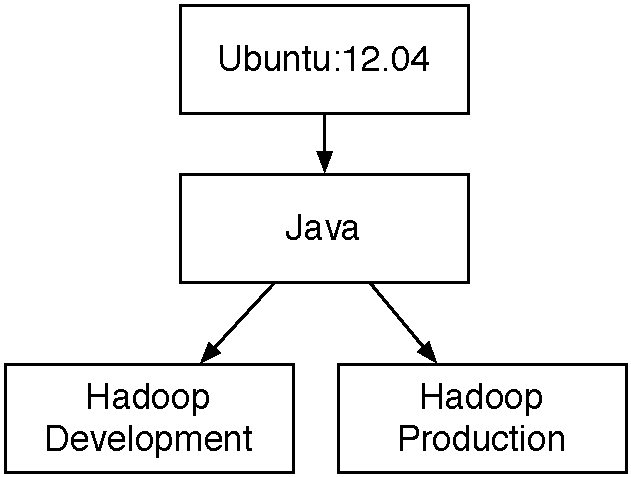
\includegraphics[width=\textwidth]{figures/hadoop-images.pdf}
  \end{columns}

\end{frame}


\begin{frame}{Developing Oracle Java7 Image}
  
  \begin{itemize}
    \item Need to base our image on a stable parent \cpause
    \item Need to carefully record our steps \cpause
    \item Want to share this with all developers \cpause
    \item Use Dockerfile! \cpause
  \end{itemize}

\end{frame}

\begin{frame}
  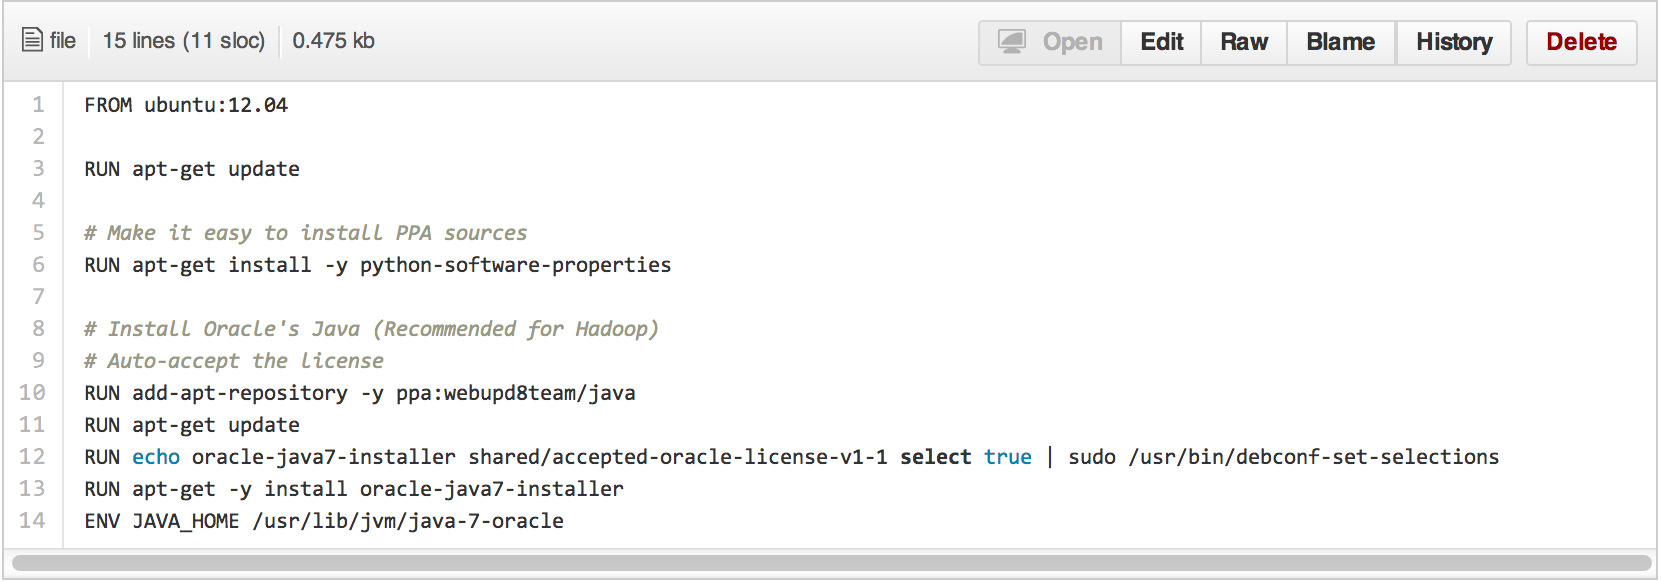
\includegraphics[width=\textwidth]{figures/dockerfile-java.png}
\end{frame}


\begin{frame}{Developing Hadoop-Dev Image}
  
  \begin{itemize}
    \item Build on top of Java7 image \cpause
    \item Install build tools \cpause
    \item Install hadoop build dependencies \cpause
    \item Run build process \cpause
    \item Of Note: This image is huge! $>1GB$ due to all the build 
    dependencies downloaded by maven \cpause
  \end{itemize}

\end{frame}

\begin{frame}{Developing Hadoop Docker}
  \centering
  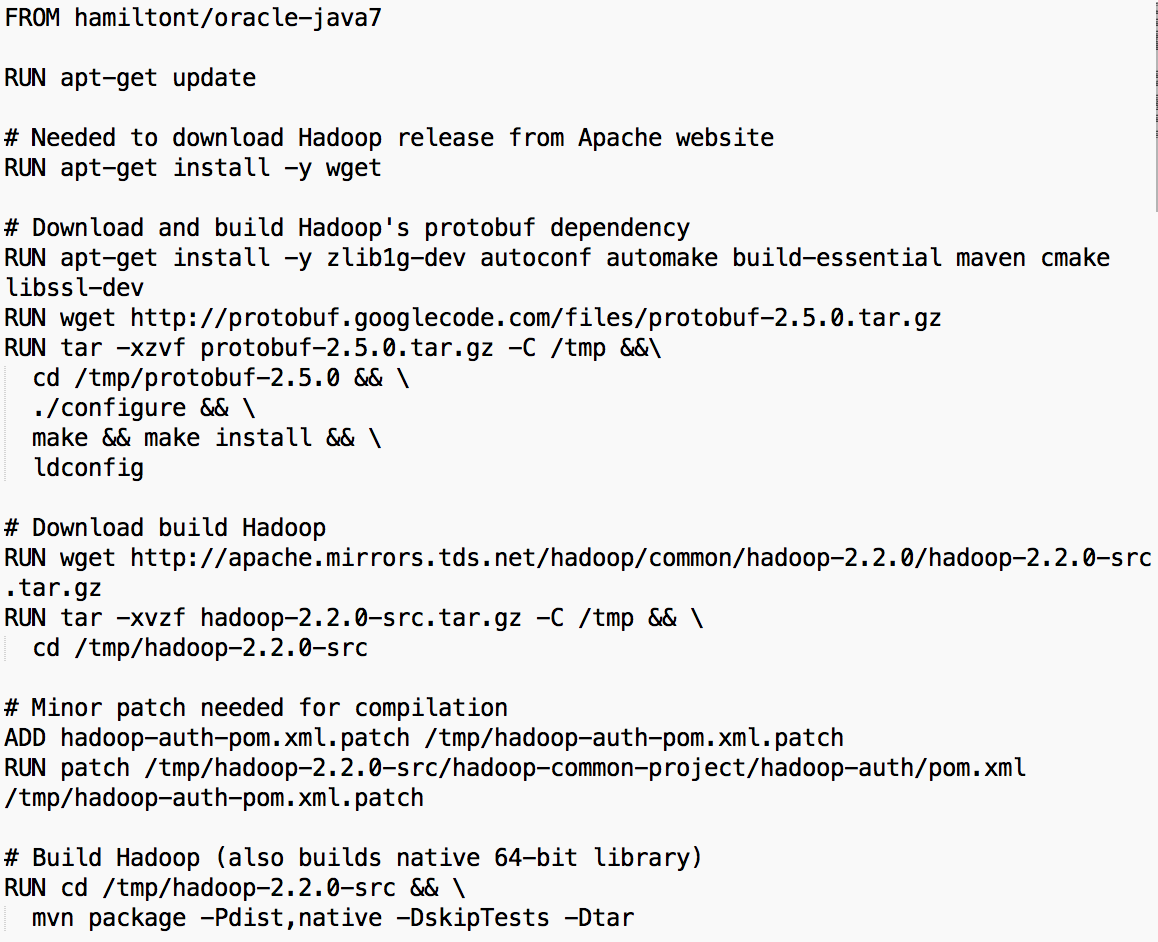
\includegraphics[width=0.7\textwidth]{figures/hadoop-dev.png}
\end{frame}

\begin{frame}{Developing Hadoop Image}
  
  \vspace{-5mm}
  \begin{itemize}
    \item Use \textbf{docker cp} to extract the tar from hadoop-dev \cpause
    \item Add that to hadoop, extract tar file \cpause
    \item Update environment PATH \cpause
    \item Install SSH server \cpause
    \item Pull in configuration files
    \item Automatically start SSH, hadoop processes \cpause
  \end{itemize}

\end{frame}

\begin{frame}{Developing Hadoop Docker}
  \centering
  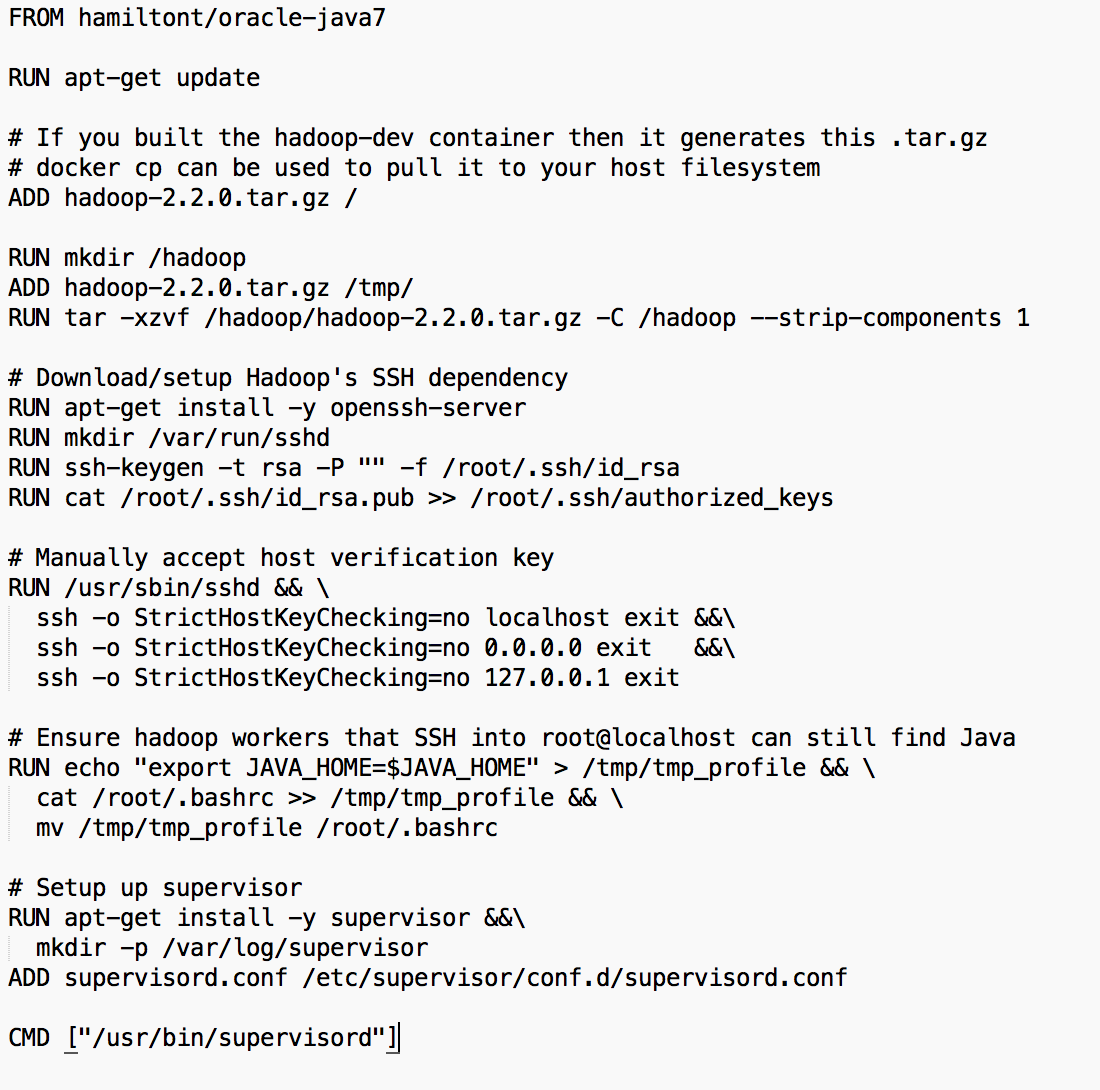
\includegraphics[width=0.8\textwidth]{figures/hadoop.png}
\end{frame}

\section{Conclusions}
\begin{frame}{Conclusions: Who and What is Docker}
  Officially, Docker is... \cpause
  \begin{itemize}
  \item Open Source, 200+ contributors \cpause
  \item Corporate parent named Docker as well ;-) \cpause
  \item Very active IRC + mailing lists \cpause
  \item A project to combine and standardize existing features of Linux \cpause
  \end{itemize}

  Unofficially, Docker is... \cpause
  \begin{itemize}
  \item The forefront in Linux Containers \cpause
  \item A huge step beyond current VM's w.r.t. machine utilization and DevOps workflow \cpause
  \item A pragmatic improvement that is here to stay \cpause
  \end{itemize}
\end{frame}

\begin{frame}{Thank You For Your Time}
  Questions? 
  \vspace{10mm}

  Please feel free to reuse/modify presentation if you wish, just remember to 
  leave my name in there somewhere. It's online at \url{https://github.com/hamiltont/intro-to-docker}
\end{frame}


\end{document}
